% a gem of a website: https://mpetroff.net/files/beamer-theme-matrix/
\documentclass[xcolor={dvipsnames,svgnames}]{beamer}
\PassOptionsToPackage{height=1cm}{beamerouterthemesidebar}
\usetheme{PaloAlto}
\usecolortheme{spruce}
\usepackage[utf8]{inputenc}
\usepackage{enumerate}
\usepackage{amsmath}
\usepackage{amsthm}
\usepackage{amssymb}
\usepackage{amsbsy}
\usepackage{amsfonts}
\usepackage{hyperref}
\usepackage{tikz}
\usepackage{verbatim}
\usepackage{mathtools}
\usepackage{macros}
\usepackage{float}
\usepackage{caption}
\usepackage[ruled,vlined,linesnumbered,algochapter]{algorithm2e}
\usepackage{subcaption}
\usepackage{xcolor,graphicx}
\usepackage{animate}
\usepackage[export]{adjustbox}
\usepackage{tikz}
\usetikzlibrary{positioning}
\setbeamertemplate{caption}[numbered]
\DeclareUnicodeCharacter{2212}{-}
\definecolor{aqua}{rgb}{0.0, 1.0, 1.0}
\definecolor{blue-green}{rgb}{0.0, 0.87, 0.87}
\definecolor{cyan-proc}{rgb}{0.0, 0.72, 0.92}
\usepackage{tikz-cd}
\usepackage{flowchart}
\usetikzlibrary{
  shapes,
  arrows.meta, % supersedes arrows
  calc,automata,positioning,fit,quotes}
  \tikzset{
  line/.style={draw, -Latex}
}
\tikzstyle{arrow} = [thick,->,>=stealth]
\captionsetup{font=scriptsize,labelfont={bf,sf}}
\captionsetup[subfigure]{font=scriptsize,labelfont=scriptsize}
\addtobeamertemplate{navigation symbols}{}{%
    \usebeamerfont{footline}%
    \usebeamercolor[fg]{footline}%
    \hspace{1em}%
    \insertframenumber/\inserttotalframenumber
}
\makeatletter
  \setbeamertemplate{sidebar \beamer@sidebarside}%{sidebar theme}
  {
    \beamer@tempdim=\beamer@sidebarwidth%
    \advance\beamer@tempdim by -6pt%
    \insertverticalnavigation{\beamer@sidebarwidth}%
    \vfill
    \ifx\beamer@sidebarside\beamer@lefttext%
    \else%
      \usebeamercolor{normal text}%
      \llap{\usebeamertemplate***{navigation symbols}\hskip0.1cm}%
      \vskip2pt%
    \fi%
}%

\AtBeginSection[]{
  \begin{frame}
  \vfill
  \centering
  \begin{beamercolorbox}[sep=8pt,center,shadow=true,rounded=true]{title}
    \usebeamerfont{title}\secname\par%
  \end{beamercolorbox}
  \vfill
  \end{frame}
}
\title{Manifold Structure of \\Artificial and Biological Neural Networks}
\author{Zhang Liu\\ Supervisor: Francesca Spagnuolo \\ Co-supervisors: Steven W.~Zucker, Luciano Dyballa}

\date{\today}
% \logo{
\includegraphics[width=.075\textwidth]{YaleNUS_workmark_solid.eps}}
\begin{document}

\begin{frame}
\titlepage
\end{frame}

\section{Motivation}

\begin{frame}{Motivation: biological vision vs computer vision}
\begin{minipage}[t]{.58\linewidth}  
\begin{figure}
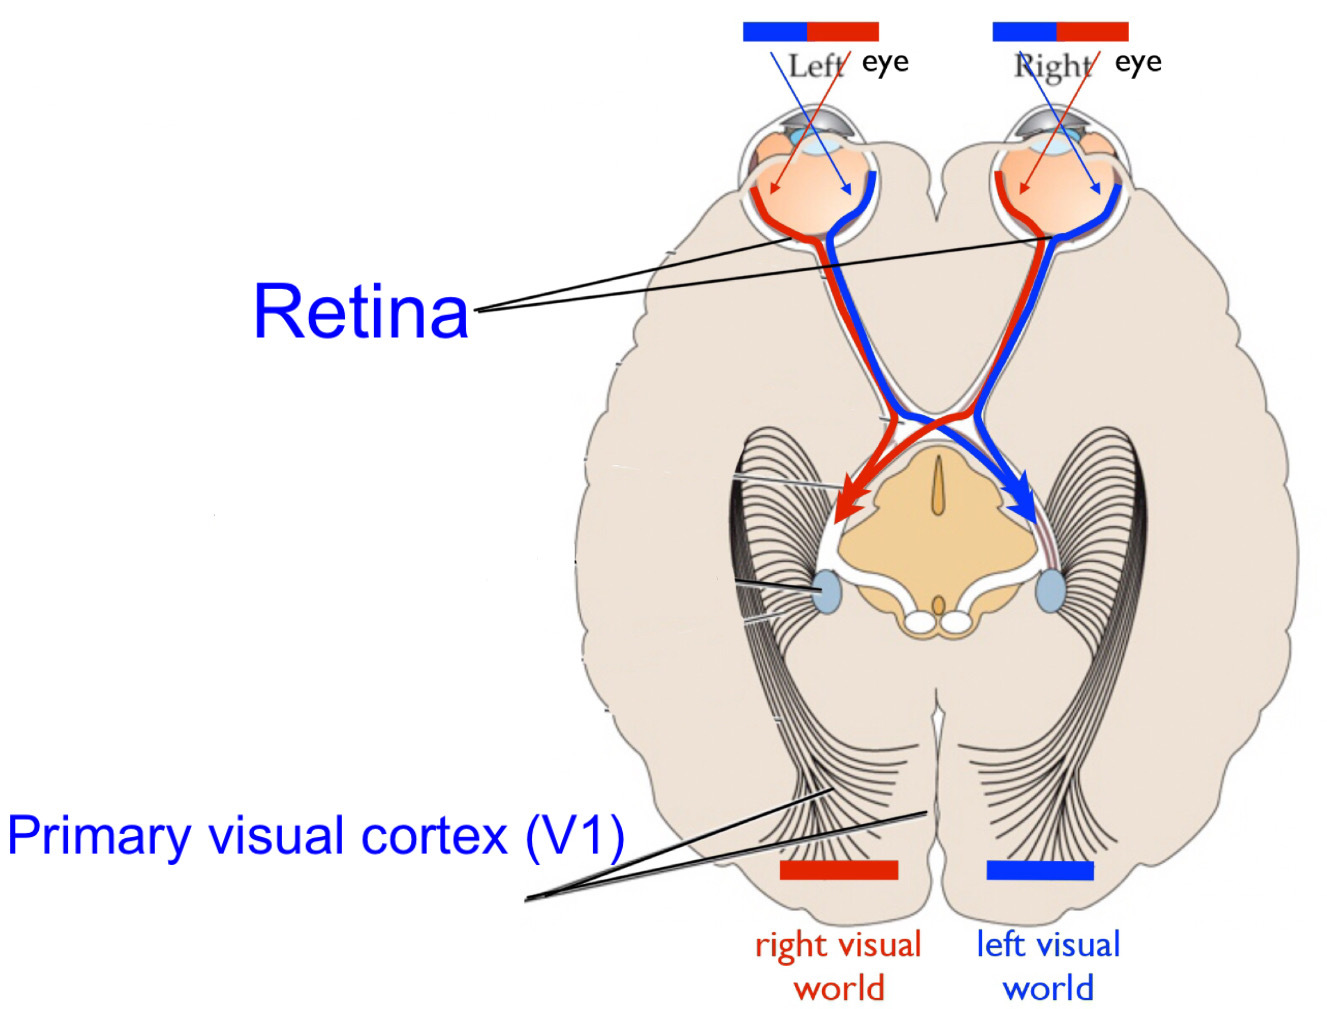
\includegraphics[width=0.6\textwidth]{figures/intro/visual-pathway.jpg}
\caption{Early visual pathway \cite{pillow_vision_2022}.}
\end{figure} 
\end{minipage}
\begin{minipage}[t]{.4\linewidth}   
\begin{figure}         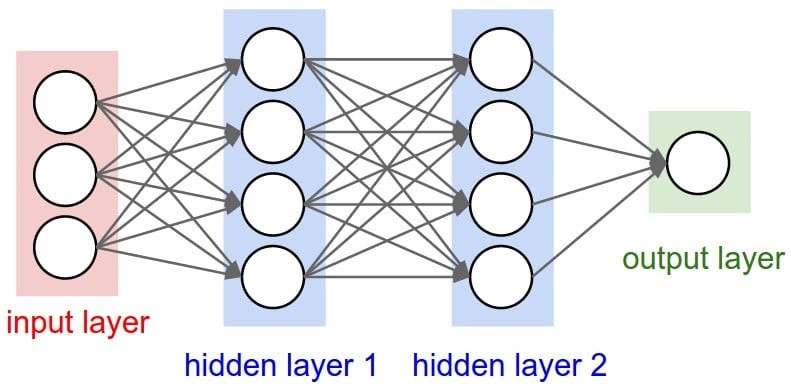
\includegraphics[width=\textwidth]{figures/intro/simple-ann.jpeg}
\caption{Illustration for a simple artificial neural network with two hidden layers.}
\end{figure} 
\end{minipage}
% (VGG16 \cite{vgg16_simonyan_very_2015}, Vision Transformer \cite{vit_dosovitskiy_image_2021}, and Convolutional Recurrent Neural Network \cite{convrnn_shi_end--end_2015})
\begin{enumerate}
    \item How do computer vision (CV) models compare to biological vision in terms of their respective \textcolor{blue}{neural circuits}?
    
     \scriptsize{\textit{\textcolor{blue}{\underline{Neural circuit}: the circuit in which the neurons connect to carry out a specific function.}}}
     
    \item  \normalsize{What specific mechanisms are important in causing such differences and/or similarities?}
\end{enumerate}
\end{frame} 

\begin{frame}{Significance}
\begin{itemize}
    \item \textbf{Neuroscience}: modeling the visual system.
    \begin{itemize}
        \item Despite decades of research, we have not fully understood the neural circuits responsible for visual perception \cite{Gwilliams221630}. 
    \end{itemize}
     
    \item \textbf{CV}: reverse-engineer desired features of biological vision.
    \begin{itemize}
        \item Neocognitron \cite{fukushima_neocognitron_1980}, CNN \cite{lenet} were inspired by earliest models of primate vision \cite{hubel_receptive_1962}.
        \item CV performs poorly on visual relational reasoning:
    \end{itemize}
    
    \begin{figure}[H]
\centering
    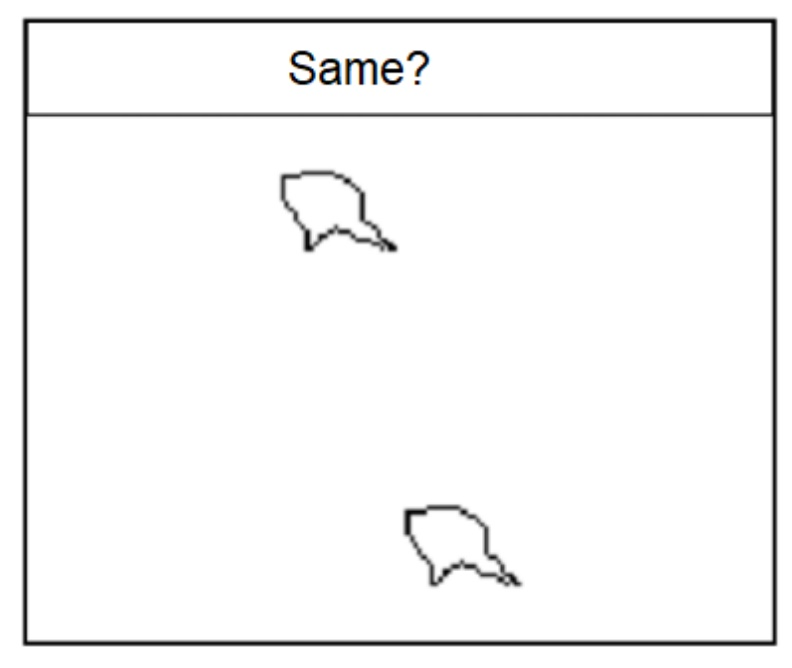
\includegraphics[width=0.4\textwidth]{figures/intro/visusal-relation.jpg}
    \caption{Same-different relations \cite{visual-categorization}, \cite{not-so-clever}.}
\end{figure}
% \hfill
% \begin{subfigure}[b]{0.45\textwidth}
% \centering
%     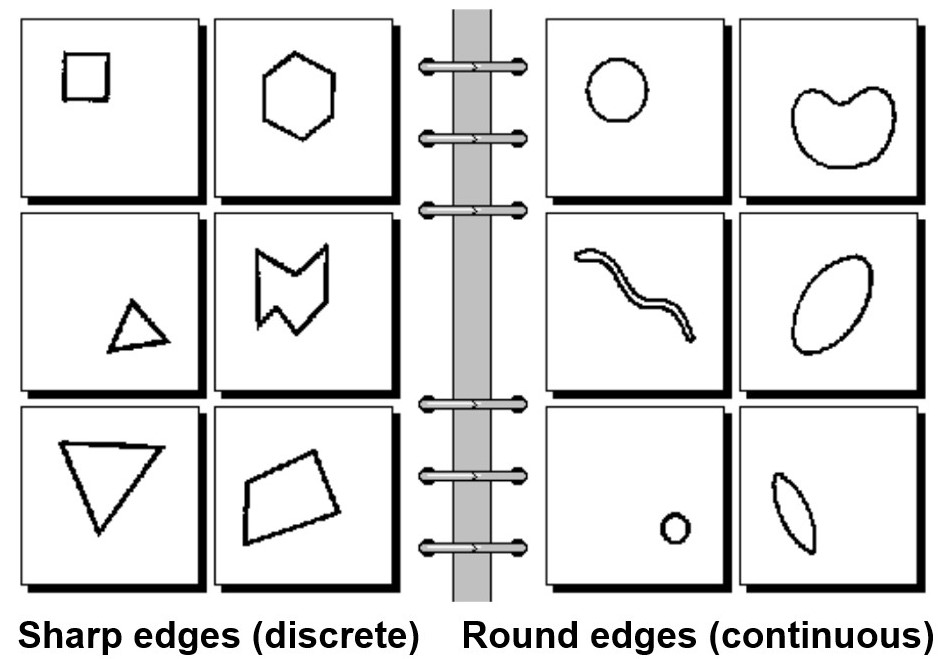
\includegraphics[width=0.8\textwidth]{figures/intro/bongard.jpg}
%     \caption{Abstraction, e.g., Bongard problems \cite{cnn-human-abstraction}.}
% \end{subfigure}
% \begin{minipage}[t]{.3\linewidth}  
% \begin{figure}
% 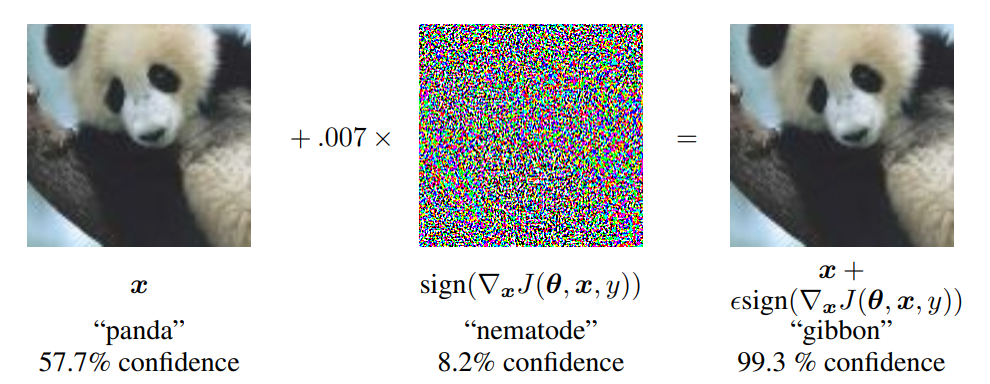
\includegraphics[width=\textwidth]{figures/intro/adversarial.PNG}
% \end{figure} 
% \end{minipage}
% \begin{minipage}[t]{.38\linewidth}   
% \begin{figure} 
% 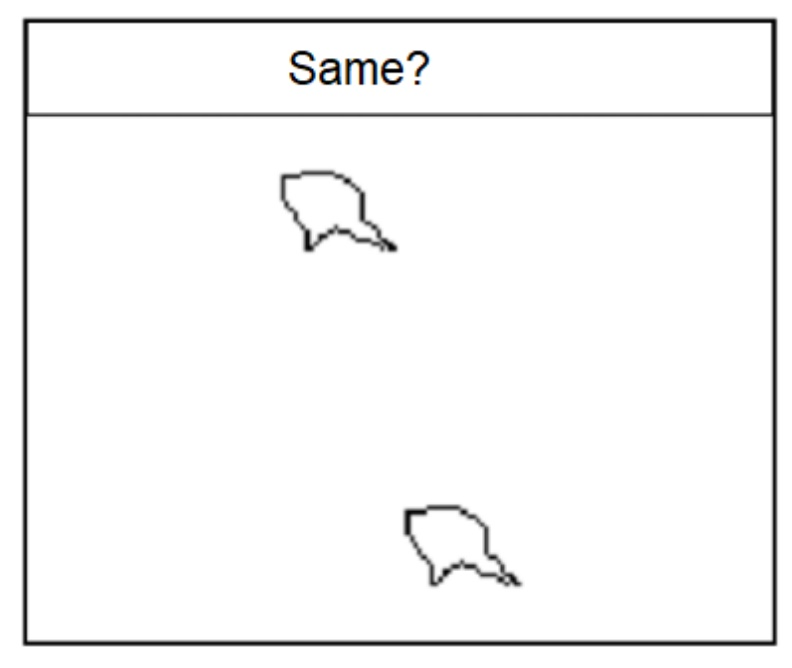
\includegraphics[width=0.6\textwidth]{figures/intro/visusal-relation.jpg}
% \end{figure} 
% \end{minipage}
    
    % our study suggests that the orientation-tilt illusion is a byproduct of neural circuits that help biological visual systems achieve robust and efficient contour detection, and that incorporating these circuits in artificial neural networks can improve computer vision.
    
\end{itemize}
\end{frame}

\section[Framework]{Framework of Comparison}

\begin{frame}{Framework of comparison}
Biological and artificial neural networks are black box problem: we do not know which are activated and how they connect to form neural circuits.
% among the billions of neurons/parameters, 
\begin{figure}[ht]
\begin{minipage}[t]{0.48\linewidth}
  \begin{enumerate} 
  \item Probe with appropriate input stimuli.
  \item Obtain neuron output. 
  \item Proxy for comparison: \textit{\textcolor{red}{neural manifold}} \\ (justified by the two-step inference).

% (1) Manifold Hypothesis.

% (2) Duality between manifold and circuit.
 \end{enumerate}
\end{minipage}
\begin{minipage}[t]{0.5\linewidth}
\centering
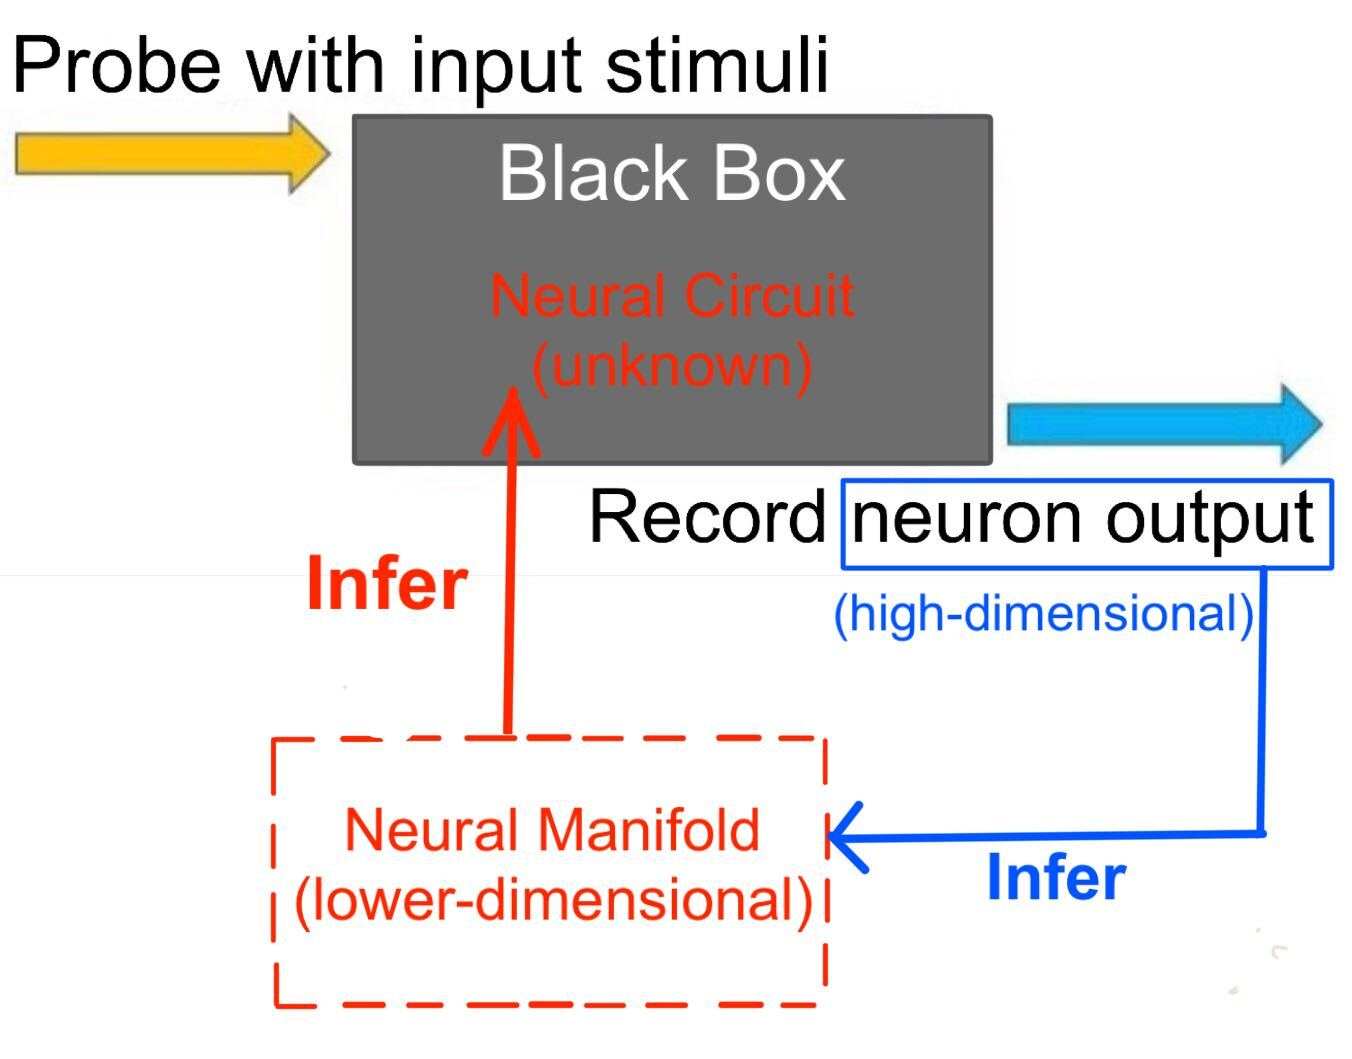
\includegraphics[%scale=1
                 width=\linewidth, valign=t]{figures/intro/black-box.jpg}
\end{minipage}
\end{figure}
\end{frame}

\begin{frame}{What is a manifold?}
\begin{defn}[Homeomorphism]
Let $f: X \to Y$ be a function between topological spaces $X$ and $Y$. If $f$ is bijective, $f$ and $f^{-1}$ are continuous, then $f$ is a \underline{homeomorphism}; $X$ and $Y$ are said to be \underline{homeomorphic}.
\end{defn}
    \begin{defn}[Manifold]
   In brief, a \underline{real $n$-dimensional manifold} is a topological space $\mathcal{M}$ for which every point $x\in\mathcal{M}$ has a neighborhood homeomorphic to Euclidean space $\RR^n$. Informally, a manifold is a topological space that locally resembles Euclidean space.
    \end{defn}
   \begin{figure}[H]
      \centering
     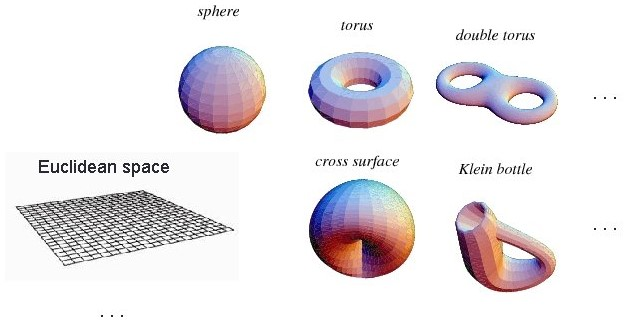
\includegraphics[width=0.4\textwidth]{figures/intro/manifold.jpg}
     \caption{Examples of $2$-dimensional manifolds.}
    \end{figure} 
\end{frame}

\begin{frame}{What is a neural manifold?}
Neural manifold is a lower-dimensional representation of the high-dimensional neural output.
    \begin{itemize}
        \item \textbf{``Manifold Hypothesis"}: natural data form lower-dimensional manifolds in their embedding space \cite{colah-manifold}.
        \item Neuroscientific justification: all possible patterns of neural output are confined to a lower-dimensional manifold \cite{gallego_neural_2017}.
    \end{itemize}
    
    \begin{minipage}[b][][b]{.65\linewidth}  
\begin{figure}
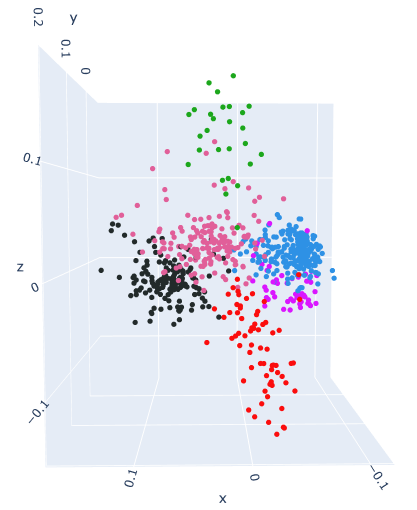
\includegraphics[width=0.35\textwidth]{figures/biological/retina-manifold.png}
     \caption{A 3D visualization of a neural manifold. Each point represents a neuron. Distance indicates how similar a pair of neurons respond.}
\end{figure} 
\end{minipage}
\begin{minipage}[b][][b]{.33\linewidth}   
\begin{figure}         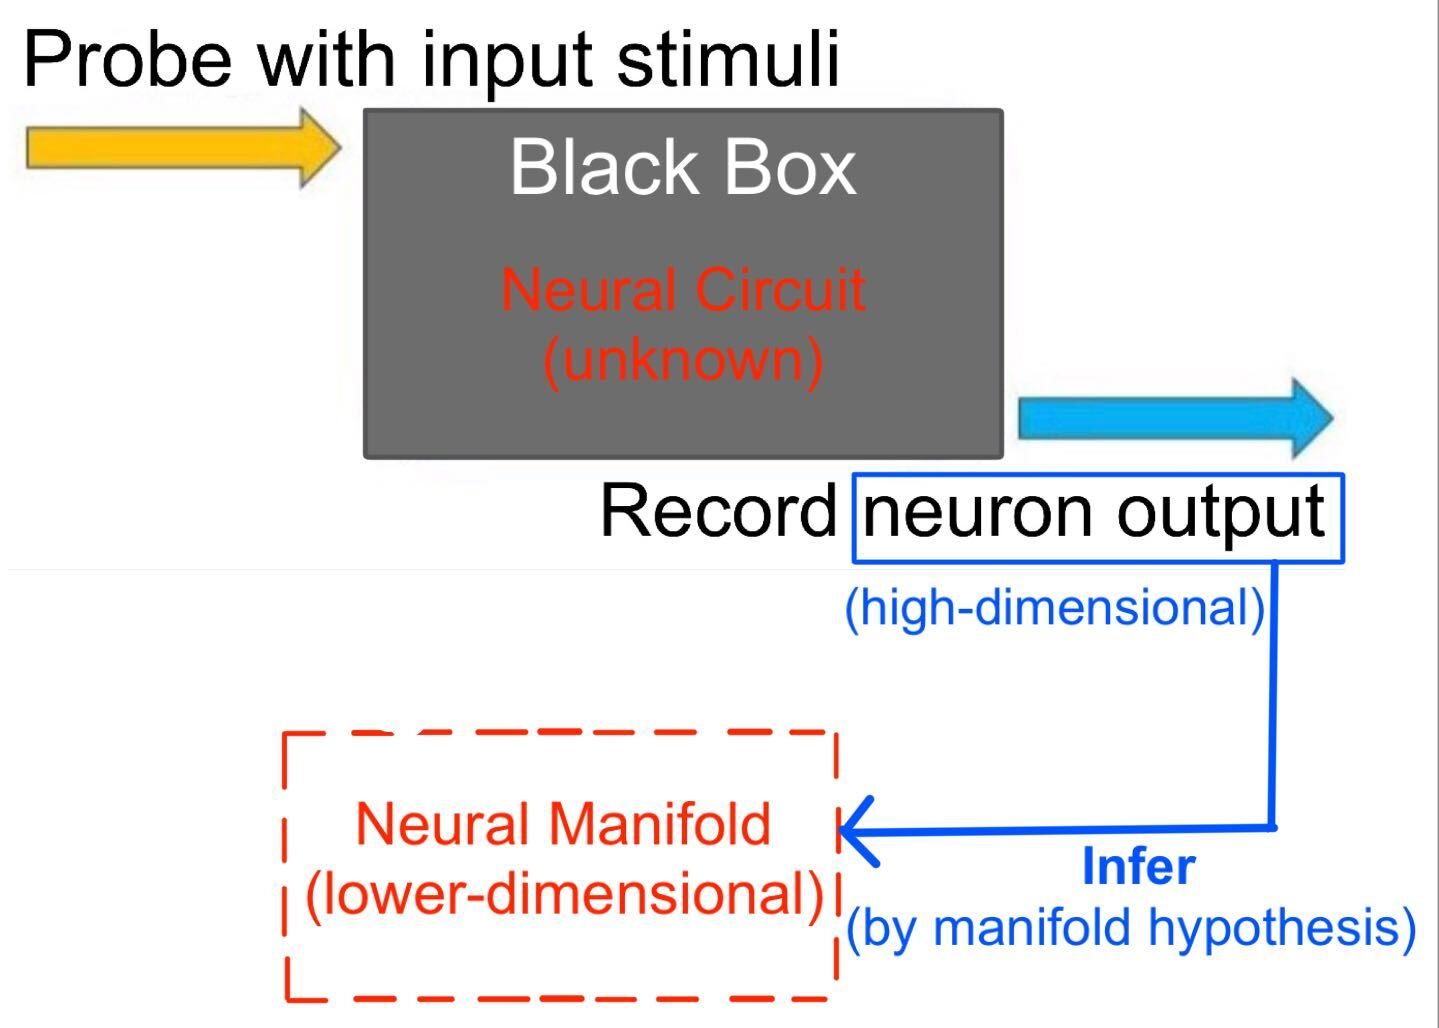
\includegraphics[width=\textwidth]{figures/intro/black-box-1.jpg}
\caption{}
\end{figure} 
\end{minipage}
\end{frame}


\begin{frame}{What can we analyze from neural manifold?}
Neural manifold is an intermediate step from the neural output towards inferring the neural circuits. This step is justified by the \textbf{duality} between network and manifold. 
    
% \begin{enumerate}[noitemsep,topsep=0pt]
%     \item from a collection of isolated neural circuits (decomposable networks), then the neurons would have distinct stimuli preferences, yielding a discontinuous neural manifold.
%     \item from overlapping neural circuits (partially decomposable networks), most neurons would respond to multiple stimuli, leading to a smooth transition in stimuli preferences and a continuous neural manifold. 
%     \item from fully connected neural circuits (non-decomposable networks),  all neurons would respond to all stimuli, and there would be no stimuli preferences across groups of neurons. This would yield a zero-dimensional (i.e., degenerate) manifold.
% \end{enumerate}

    \begin{minipage}[b][][b]{.65\linewidth}  
\begin{figure}
    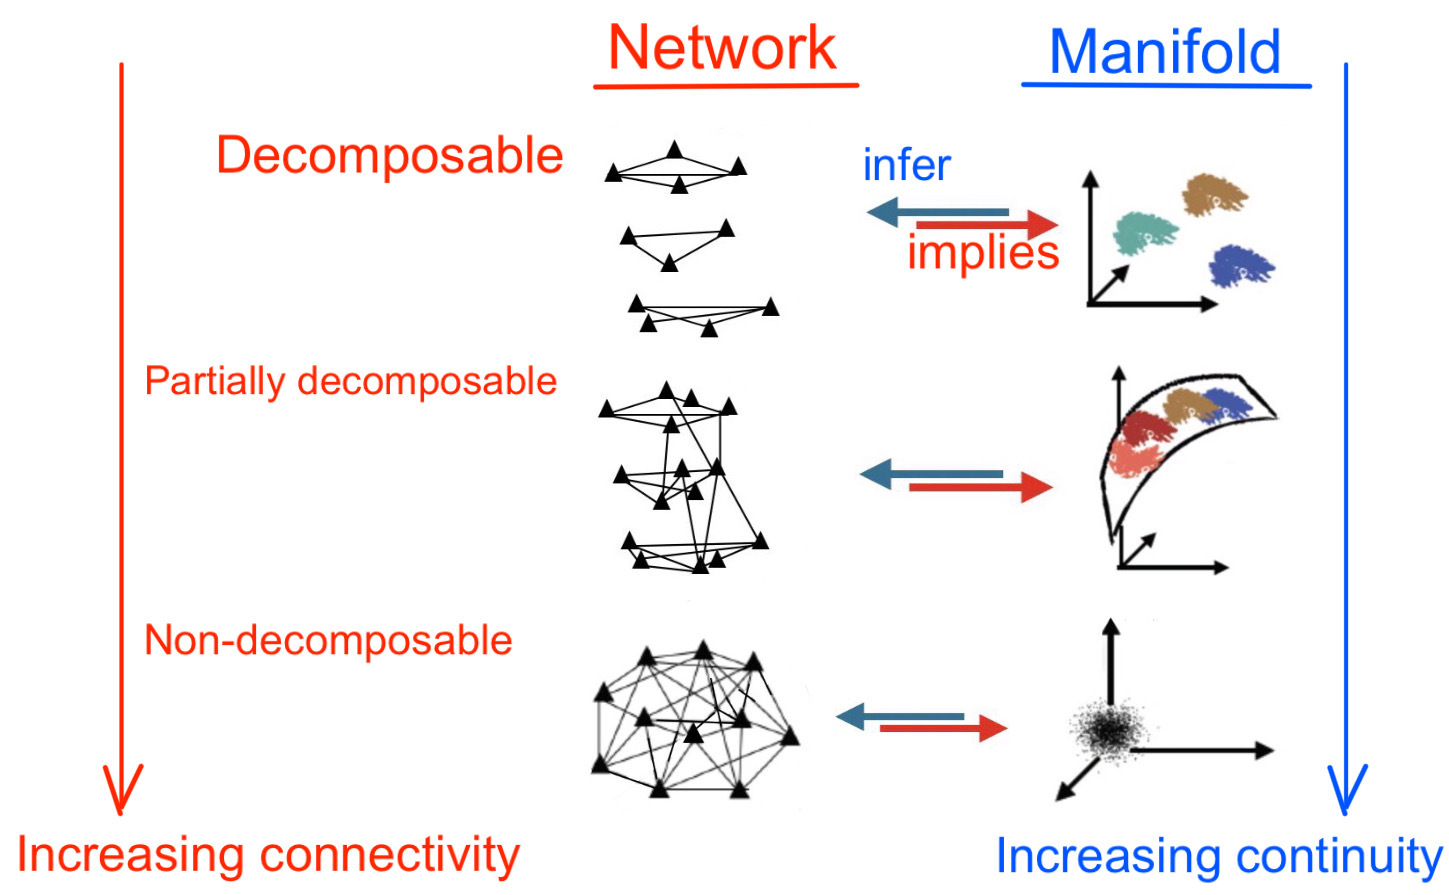
\includegraphics[width=\textwidth]{figures/intro/networks-manifolds.jpg}
    \caption{Duality between network and manifold.}
\end{figure} 
\end{minipage}
\begin{minipage}[b][][b]{.33\linewidth}   
\begin{figure}         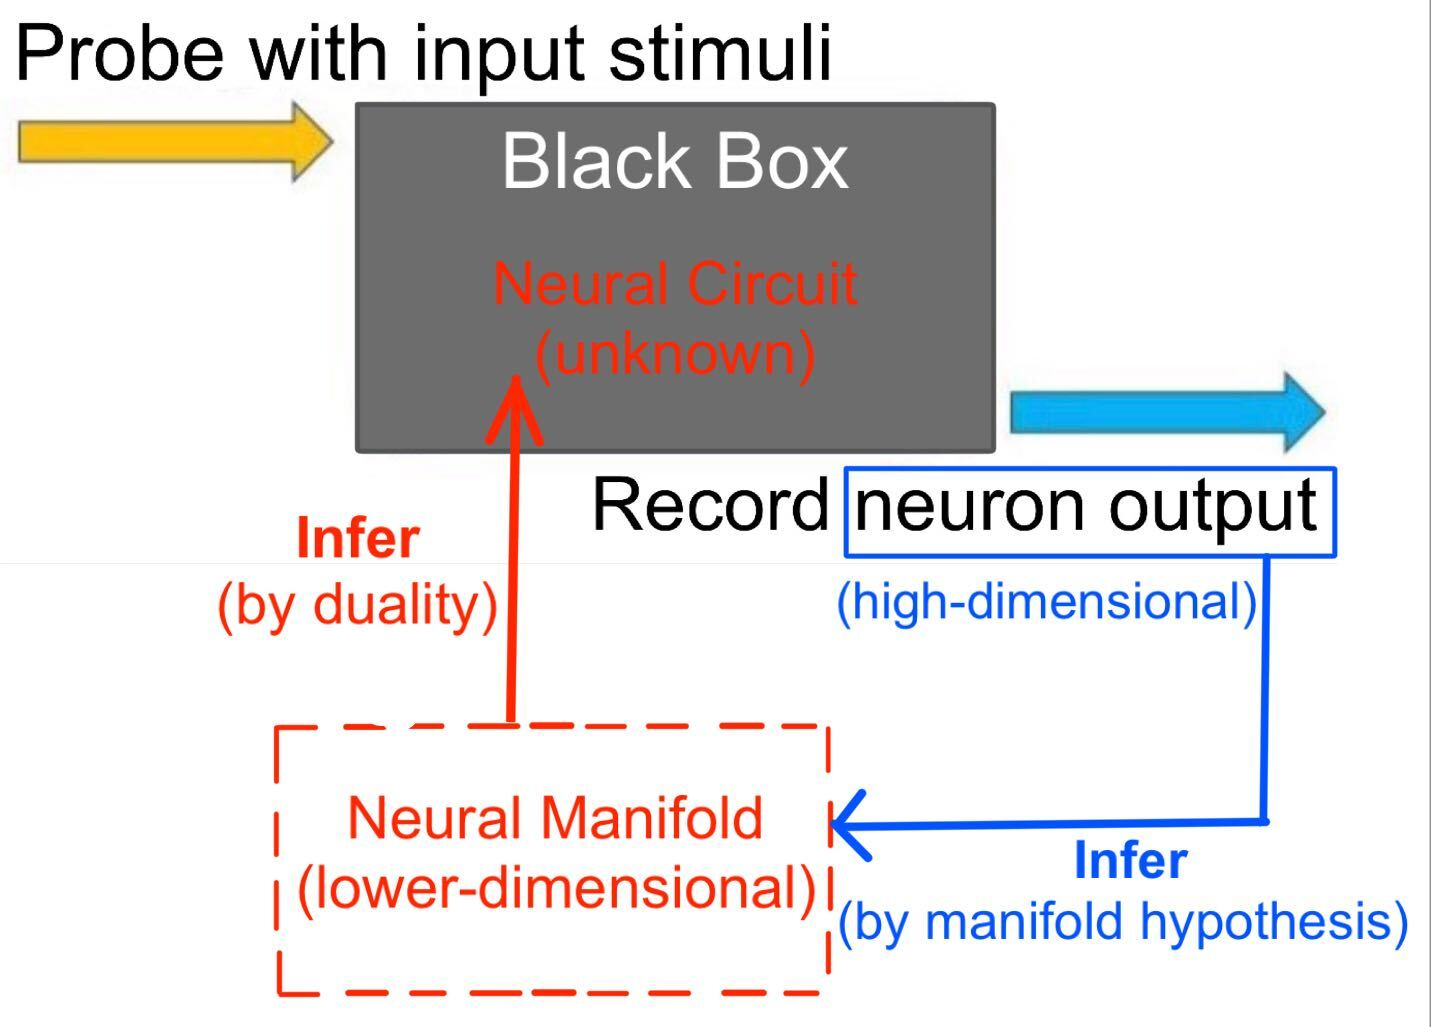
\includegraphics[width=\textwidth]{figures/intro/black-box-2.jpg}
\end{figure} 
\end{minipage}

\end{frame}

\begin{frame}{Framework of comparison}
\begin{table}[H]
\centering
 \noindent\resizebox{\textwidth}{!}{\begin{tabular}{|l|l|l|}
\hline
        & Biological & Artificial     \\ \hline
Models   & retina, V1      & CNN, ViT, RNN \\\hline
Input & flow stimuli \cite{visual-flow}  & ImageNet images \cite{deng2009imagenet} \\ \hline
Output & single-neuron recording  & artificial neuron output \\ \hline
\end{tabular}}
\caption{Summary of comparison.} 
\end{table} 

\begin{minipage}[t]{.5\linewidth}  
    \begin{figure}
            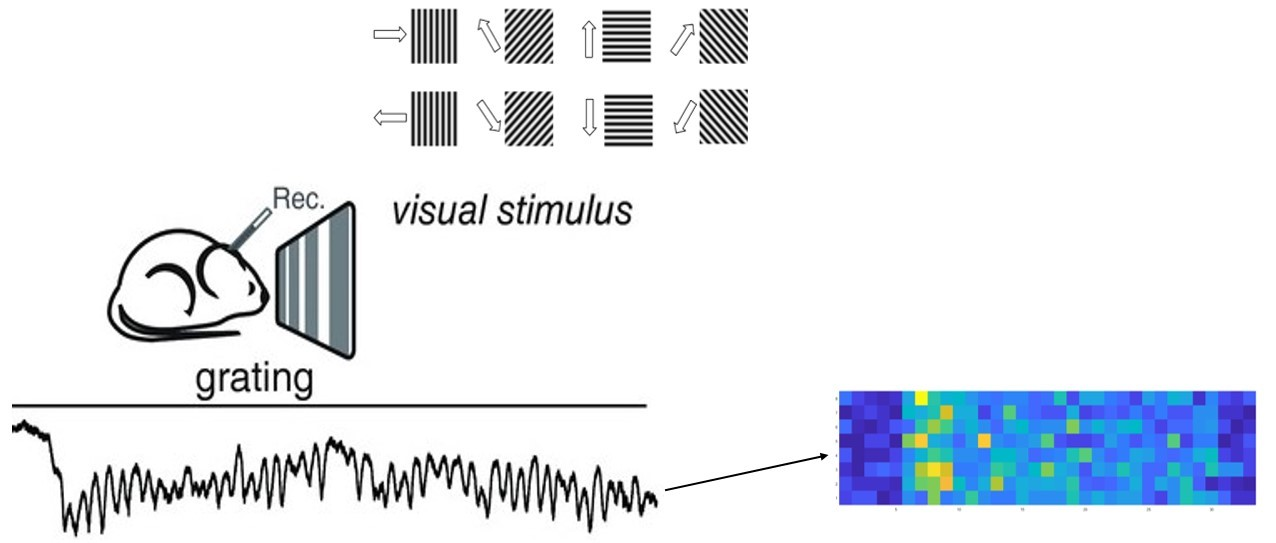
\includegraphics[width=\textwidth]{figures/biological/biological-input-output.jpg}
            \caption{Input and output in biological neural networks.}
        \end{figure} 
    \end{minipage}
      \begin{minipage}[t]{.45\linewidth}   
      \begin{figure}         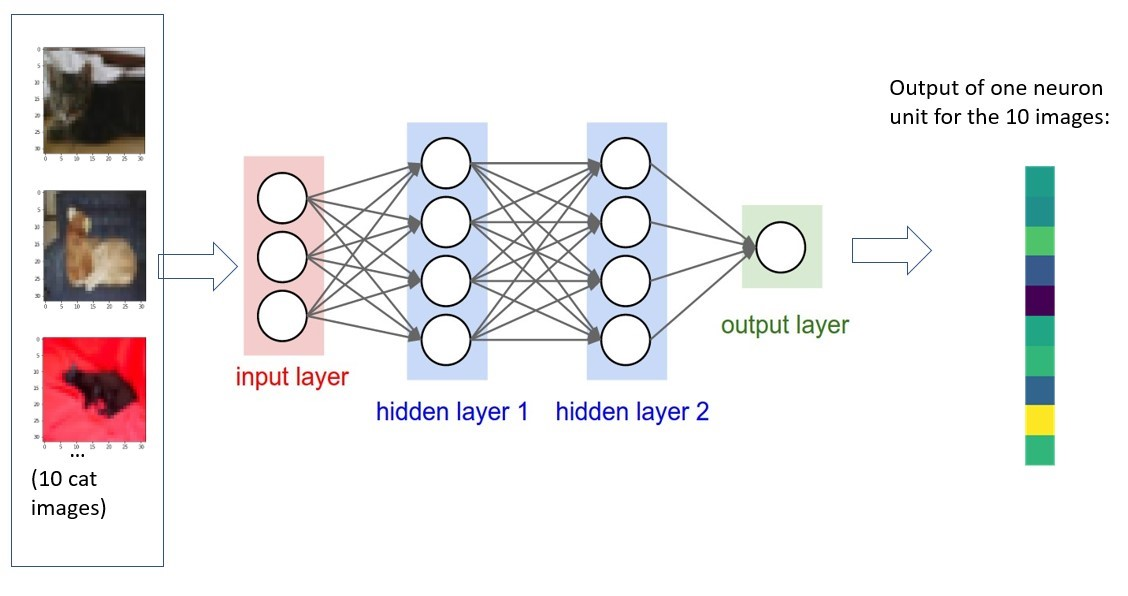
\includegraphics[width=\textwidth]{figures/artificial/artificial-input-output.jpg}
      \caption{Input and output in artificial neural networks.}
            \end{figure} 
    \end{minipage}
    
\end{frame}

\begin{frame}{Starting point: retina vs V1}
Neural manifold for V1 is much more continuous than that for the retina, suggesting higher connectivity in the neural circuit of V1. 

\textbf{Questions:} Do artificial neural networks in computer vision form continuous manifold like V1 or discontinuous manifold like the retina? 

    \begin{minipage}[t]{.48\linewidth}  
    \begin{figure}
            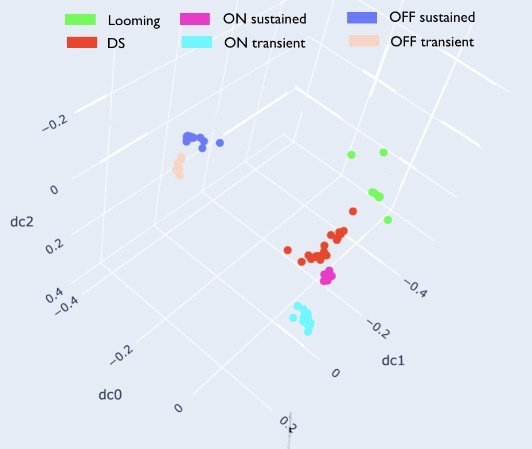
\includegraphics[width=0.65\textwidth]{figures/biological/retina-manifold-luciano.jpg}
            \caption{Retina neural manifold \cite{dyballa_manifold_2021}.}
        \end{figure} 
    \end{minipage}
      \begin{minipage}[t]{.48\linewidth}   
      \begin{figure}         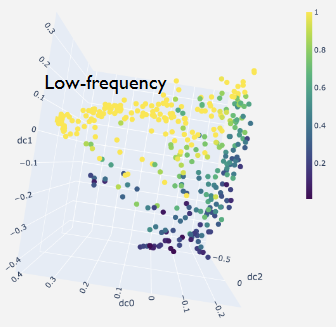
\includegraphics[width=0.55\textwidth]{figures/biological/v1-manifold-luciano.PNG}
      \caption{V1 neural manifold \cite{dyballa_manifold_2021}.}
            \end{figure} 
    \end{minipage}
\end{frame}

\section[Methods]{Methods}
\begin{frame}{Dimensionality reduction}
The neuron output is encoded in neural tensor:
\begin{defn}[Neural tensors]
    Each \underline{neural tensor} encodes the output of $N$ neurons to $K$ flow stimuli over $T$ time steps and is a $3$-way $N$-by-$K$-by-$T$ tensor. An $N$-way tensor is an element of the tensor product of $N$ vector spaces. A $2$-way tensor is a matrix.
\end{defn}
The neural tensor has a high-dimensional representation ($N$, $K$, $T$ are very large) and its structure cannot be visualized directly. 

    \begin{figure}[H]
        \centering
            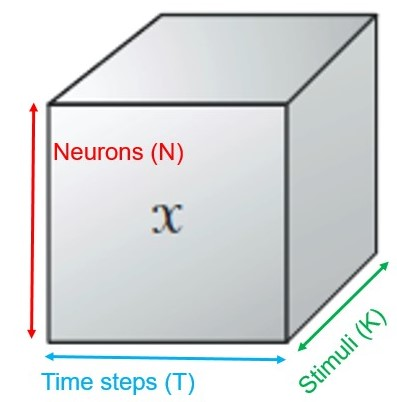
\includegraphics[width=0.2\textwidth]{figures/linear/neural-tensor.jpg}
            \caption{Visualization of the neural tensor.}
        \end{figure} 
\end{frame}

\begin{frame}{Dimensionality reduction}

\begin{enumerate}
    \item We use Tensor CANDECOMP/PARAFAC (CP) decomposition with nonnegativity constraint, called "Nonnegative Tensor Factorization (NTF)."
    \item Apply NTF on the neural tensor to get the \textcolor{red}{neural factors}.
    % , using Tensor Toolbox in MATLAB \cite{tensortoolbox} and tensortools in Python \cite{williams_unsupervised_2018}.
    \item Concatenate the \textcolor{red}{neural factors} to get an $N$-by-$R$ neural matrix.
\end{enumerate}
    \begin{figure}[H]
        \centering
            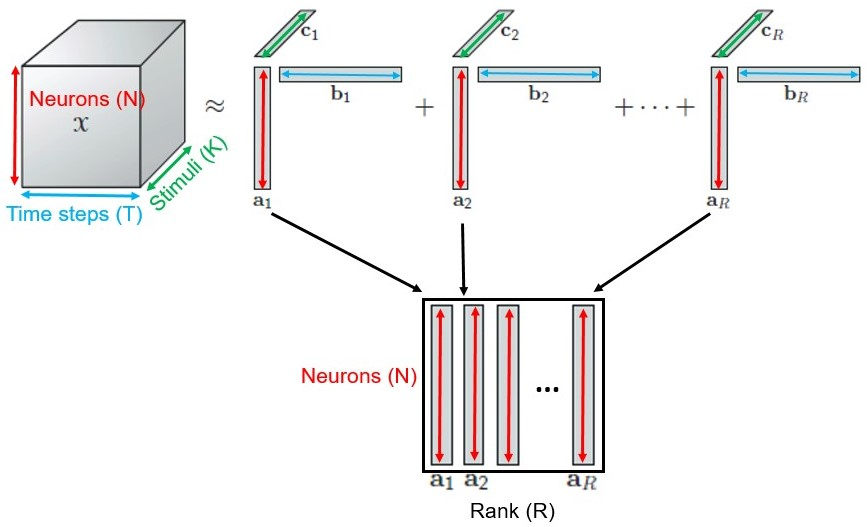
\includegraphics[width=0.7\textwidth]{figures/linear/cp-decomp-marked.jpg}
        \end{figure} 
\end{frame}

\begin{frame}{Dimensionality reduction}
\begin{enumerate}\setcounter{enumi}{3}
    \item Apply PCA on the neural matrix (consisting of \textcolor{red}{neural factors}) to get the orthogonal principal components. This step has the same effect as other manifold learning methods such as diffusion map. 
    \item Use the first three principal components to plot the 3D projection. This provides a 3D visualization of the neural manifold. 
    \begin{figure}
    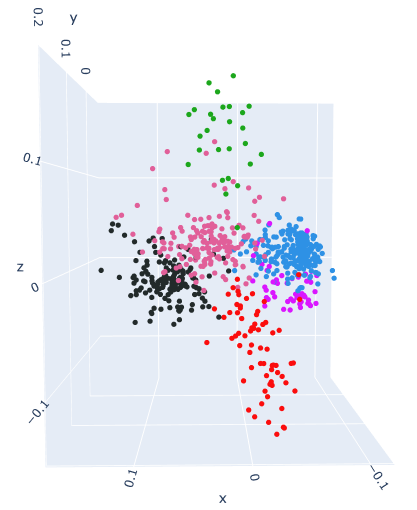
\includegraphics[width=0.35\textwidth]{figures/biological/retina-manifold.png}
     \caption{A 3D visualization of a neural manifold.}
\end{figure} 
\end{enumerate}
\end{frame}

\begin{frame}{Quantifying continuity: mean flow ratio ($\phi_G$)}
\begin{itemize}
    \item We adapt the mean flow ratio (MFR) developed in \cite{dyballa_manifold_2021} to quantify the continuity of a given neural manifold.
    \item $\phi_G \in [0,1]$ and the greater the $\phi_G$ is, the more continuous the neural manifold is, and vice versa.
\end{itemize}
  \begin{figure}[H]
        \centering
         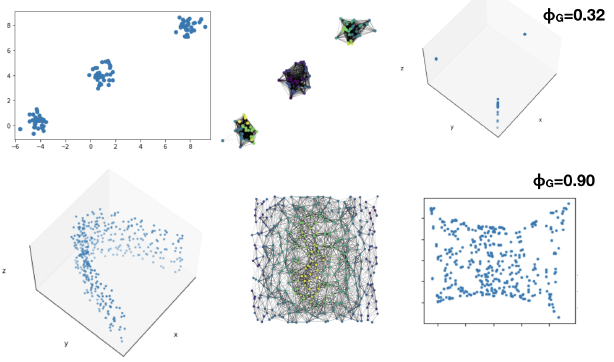
\includegraphics[width=0.8\textwidth]{presentation/embeddings/mean-flow-ratio.PNG}
            \caption{Intuition for mean flow ratio. (Adapted from \cite{dyballa_manifold_2021}.)}
        \end{figure} 
\end{frame}

\section[Results: biological]{Results: Biological Neural Networks}

\begin{frame}{Retina: neural factors}

  \begin{figure}[H]       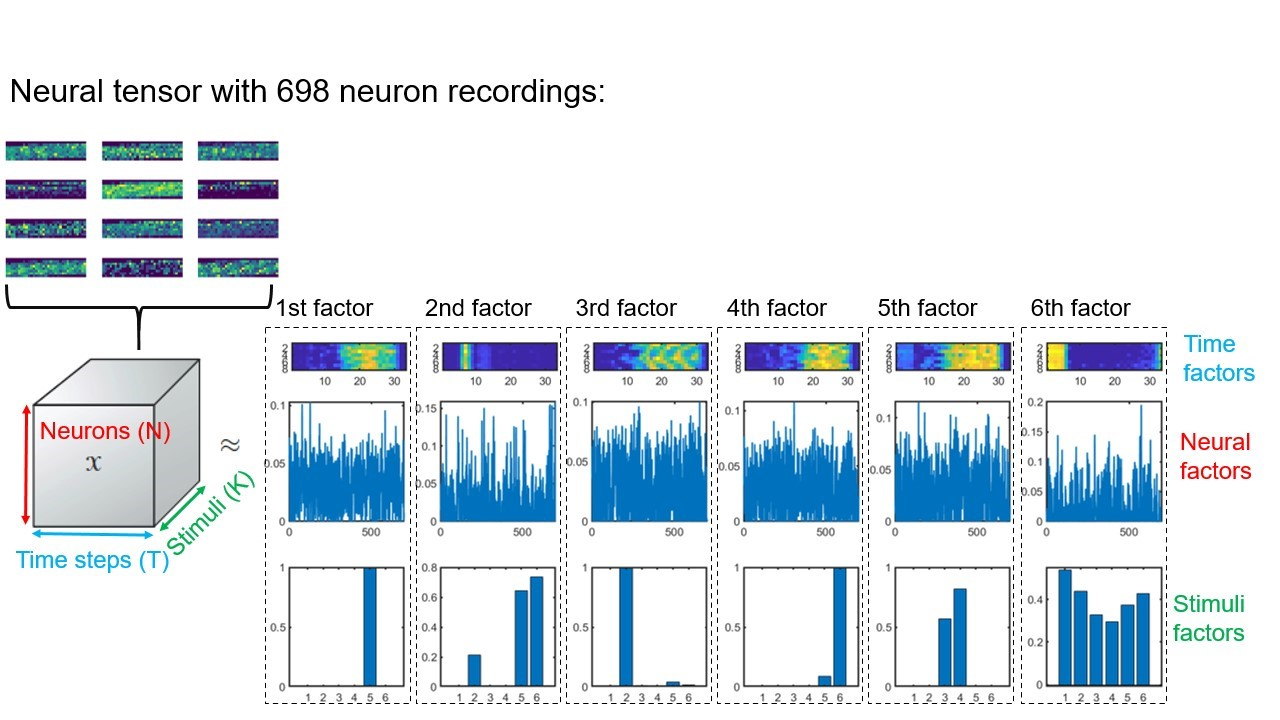
\includegraphics[width=\textwidth]{figures/biological/retina-factors.jpg}
  \caption{Visualizing the resulting tensor factors.}
\end{figure} 
\end{frame}

\begin{frame}{Retina: neural manifold}
\begin{itemize}
    \item Neurons with similar firing patterns organize into distinct clusters.
    \item Retina neural manifold is discontinuous.
    \item Retina neural circuit form isolated subcircuits with low inter-connectivity.
\end{itemize}
         \begin{figure}[H]
        \centering
            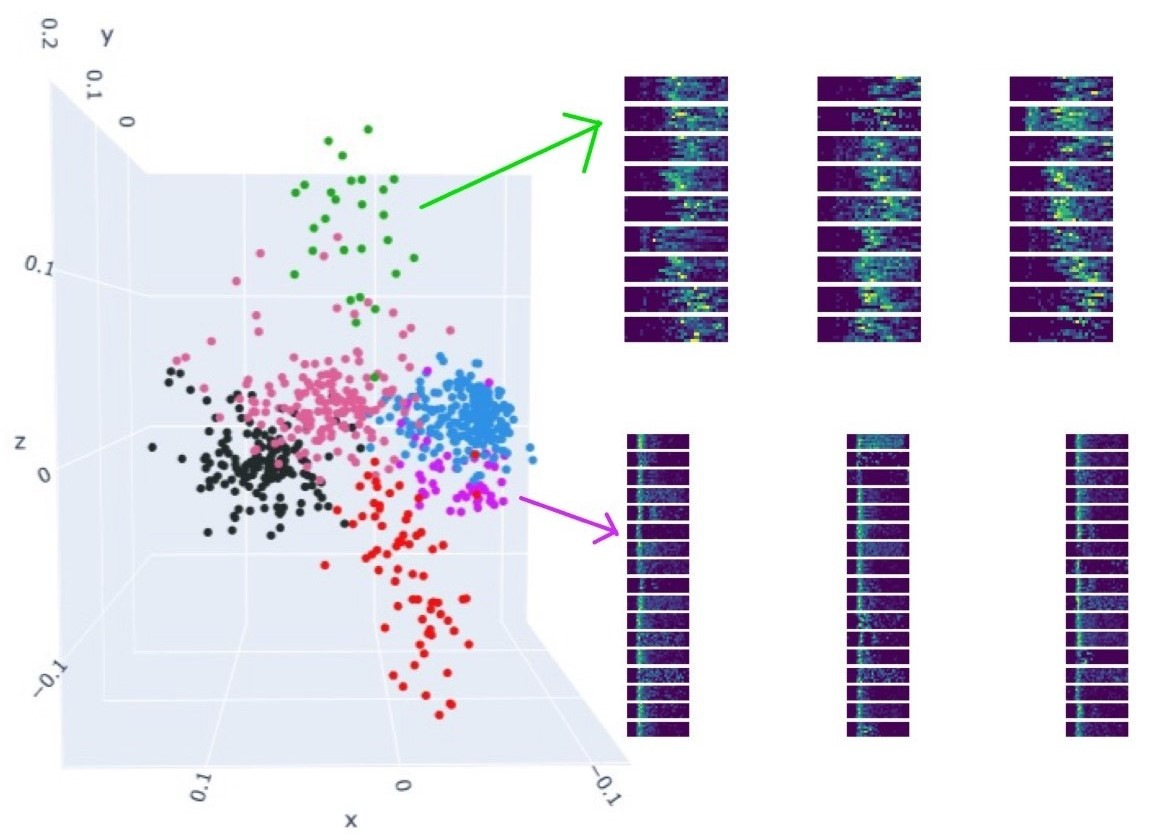
\includegraphics[width=0.75\textwidth]{figures/biological/retina-manifold-with-psth.jpg}
        \end{figure} 
\end{frame}


\section[Results: artificial]{Results: Artificial Neural Networks}

\begin{frame}{CNN: algorithm for sampling neuron output}
\begin{itemize}
    \item Convolutional layer has several feature maps, each corresponding to a filter of certain size and weights. 
    \item Neurons in the same feature map share the same weights and each attends to a subregion of the image (within its receptive field).
\end{itemize}
    \begin{minipage}[t]{.45\linewidth} 
     \begin{figure}[H]
        \centering
            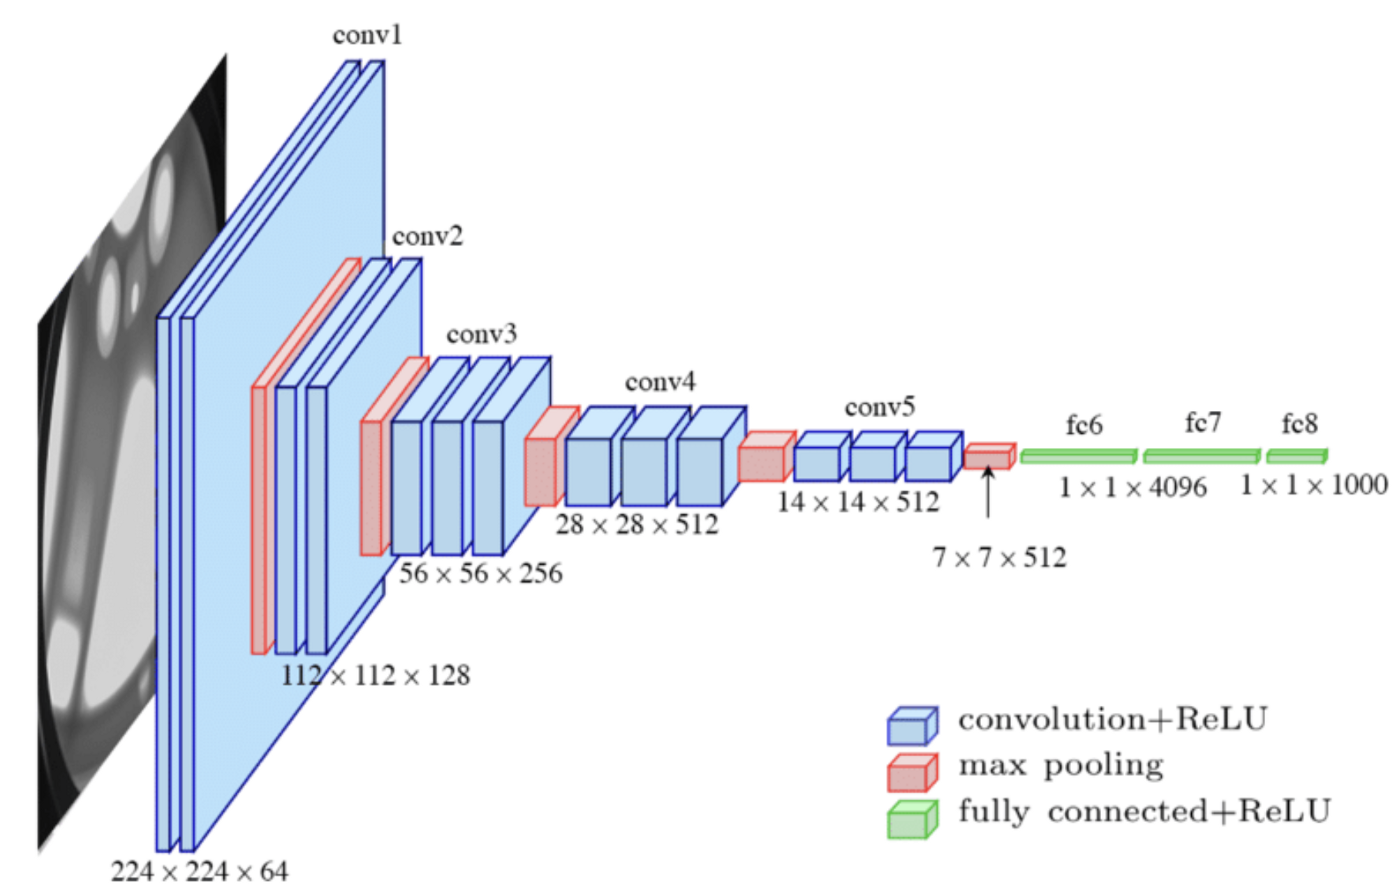
\includegraphics[width=\textwidth]{figures/artificial/vgg16-model.png}
             \caption{Structure of VGG16.}
        \end{figure} 
        \end{minipage}
    \begin{minipage}[t]{.45\linewidth} 
        \begin{figure}
    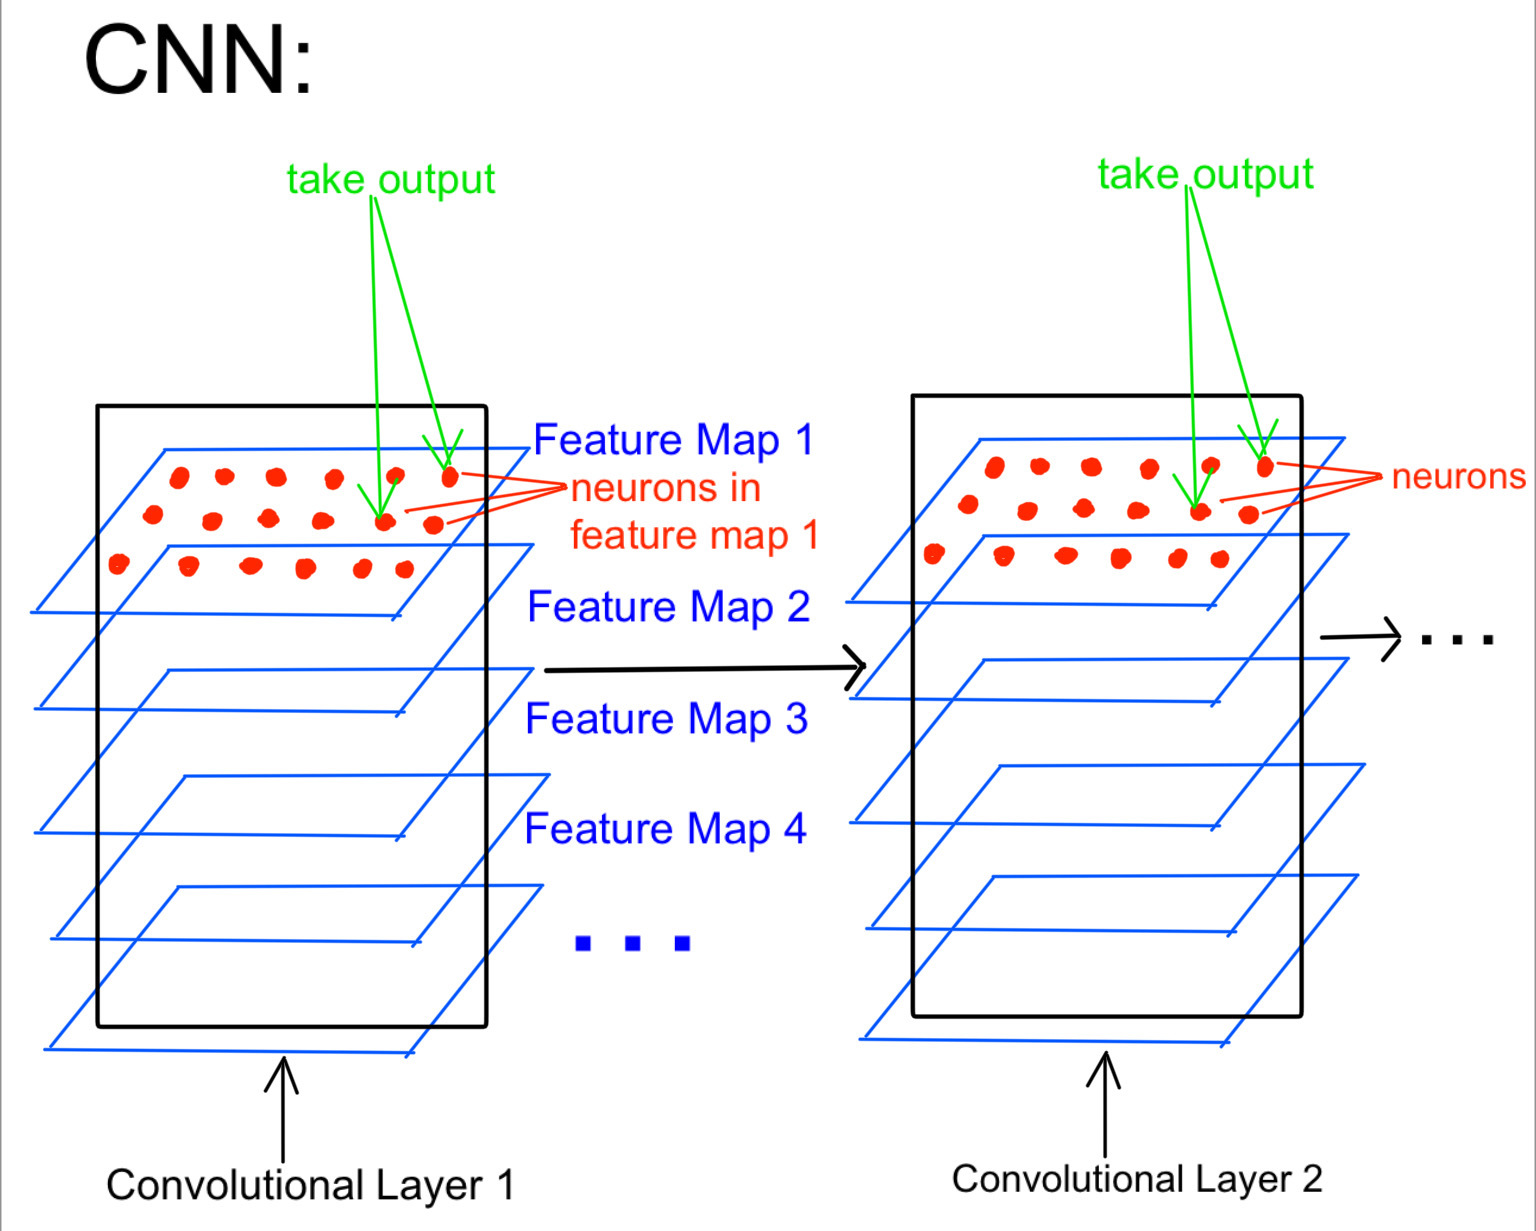
\includegraphics[width=0.8\textwidth]{figures/artificial/cnn-tensor.jpg}
    \caption{Taking neuron output from VGG16.}
\end{figure}
\end{minipage}
\end{frame}

\begin{frame}{CNN: neural manifold}
\begin{itemize}
    \item Neurons from the same feature map form distinct clusters.
    \item CNN neural manifold is discontinuous.
    \item CNN neural circuit form isolated subcircuits with low inter-connectivity.
    \item From shallow to deep layers, the clusters become more diffused but still distinct. 
\end{itemize}

    \begin{minipage}[t]{.5\linewidth}  
    \begin{figure}
            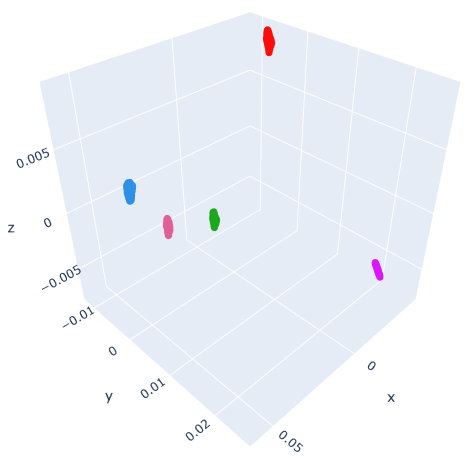
\includegraphics[width=0.7\textwidth]{figures/embeddings/VGG16-2D-block1.png}
             \caption{CNN neural manifold by sampling neuron output from convolutional layers in block 1 (shallow).}
        \end{figure} 
    \end{minipage}
      \begin{minipage}[t]{.48\linewidth}   
      \begin{figure}         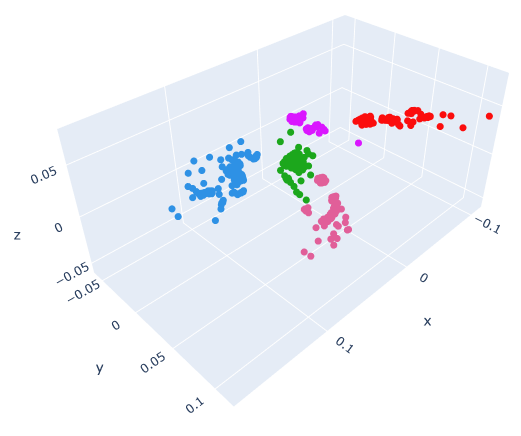
\includegraphics[width=0.8\textwidth]{figures/embeddings/VGG16-2D-block3.png}
      \caption{CNN neural manifold by sampling neuron output from convolutional layers in block 3 (deep).}
            \end{figure} 
    \end{minipage}
\end{frame}
% \begin{frame}{CNN: spatial ordering of neurons is preserved}
% Within each cluster, the spatial ordering of neurons' receptive fields are continuously mapped onto the manifold. 
%     \begin{minipage}[t]{.45\linewidth}  
%     \begin{figure}
%             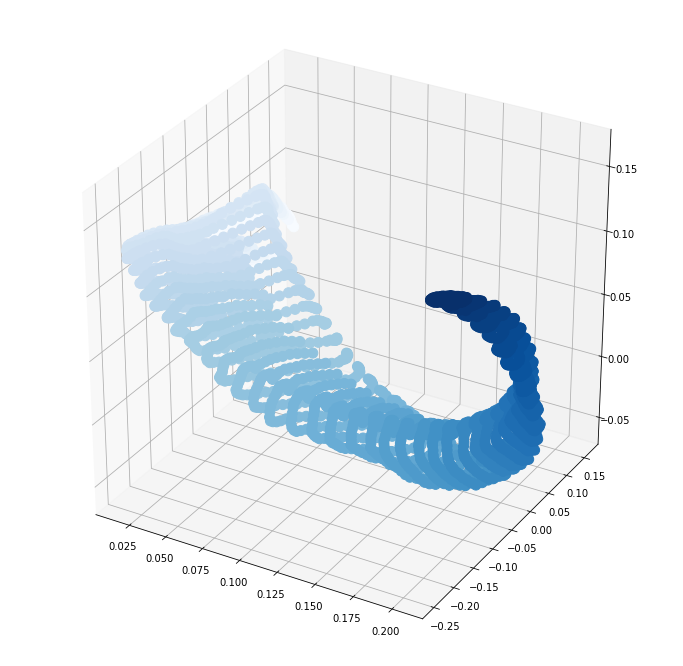
\includegraphics[width=0.7\textwidth]{figures/embeddings/vgg16-spatial1.png}
%             \caption{First cluster of neurons organized by vertical order.}
%         \end{figure} 
%     \end{minipage}
%       \begin{minipage}[t]{.45\linewidth}   
%       \begin{figure}         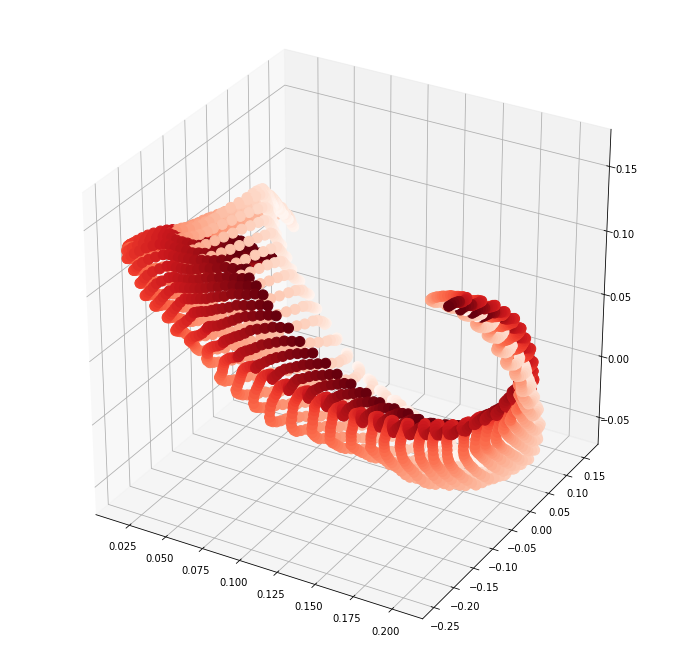
\includegraphics[width=0.7\textwidth]{figures/embeddings/vgg16-spatial2.png}
%       \caption{First cluster of neurons organized by horizontal order.}
%             \end{figure} 
%     \end{minipage}
% \end{frame}
\begin{frame}{Vision Transformer (ViT)}
Inspired by Transformer for NLP applications: an image is a sequence of 16-by-16 ``words." The main mechanism in ViT is the self-attention in the encoder layer.
      \begin{figure}[H]
        \centering
            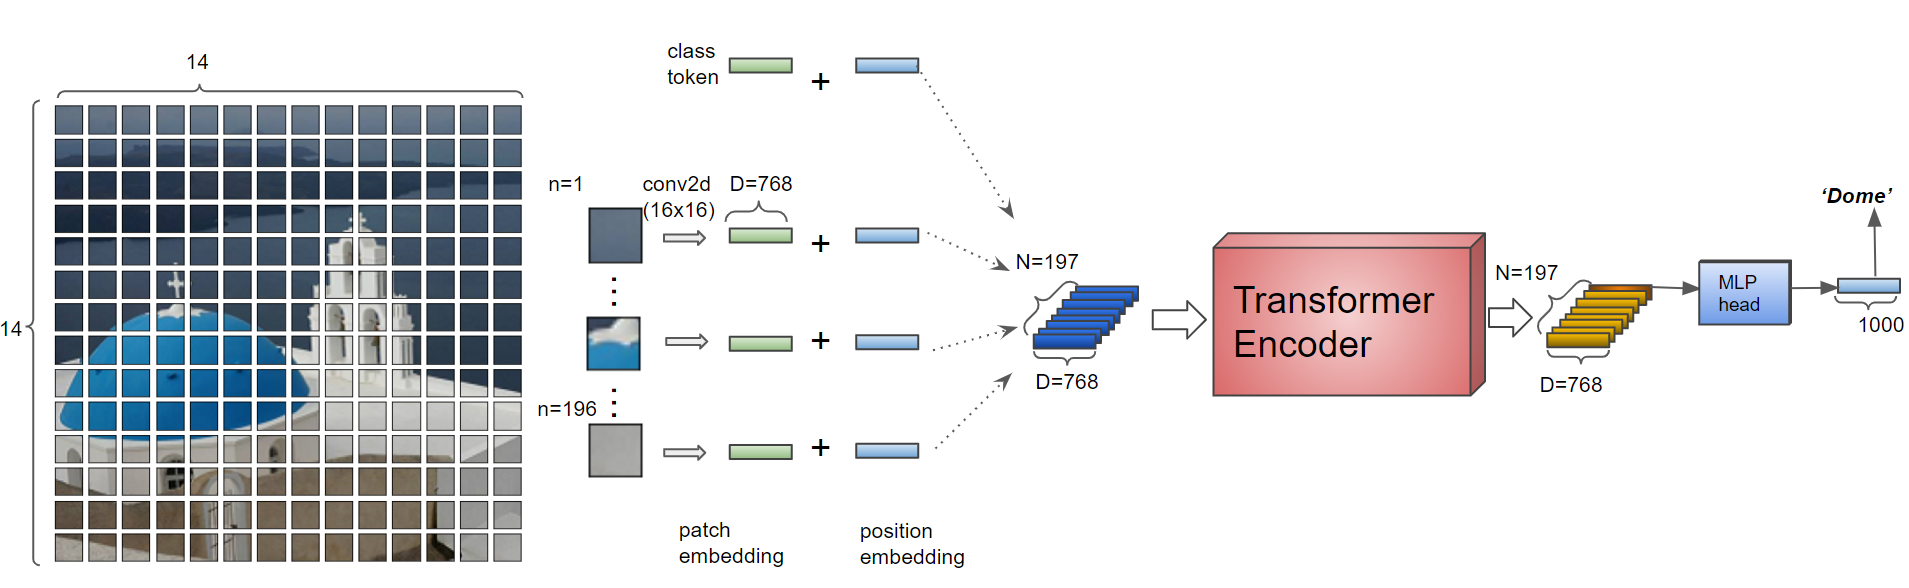
\includegraphics[width=0.8\textwidth]{figures/artificial/vit_input.png}
        \end{figure} 
        \begin{figure}[H]
        \centering
            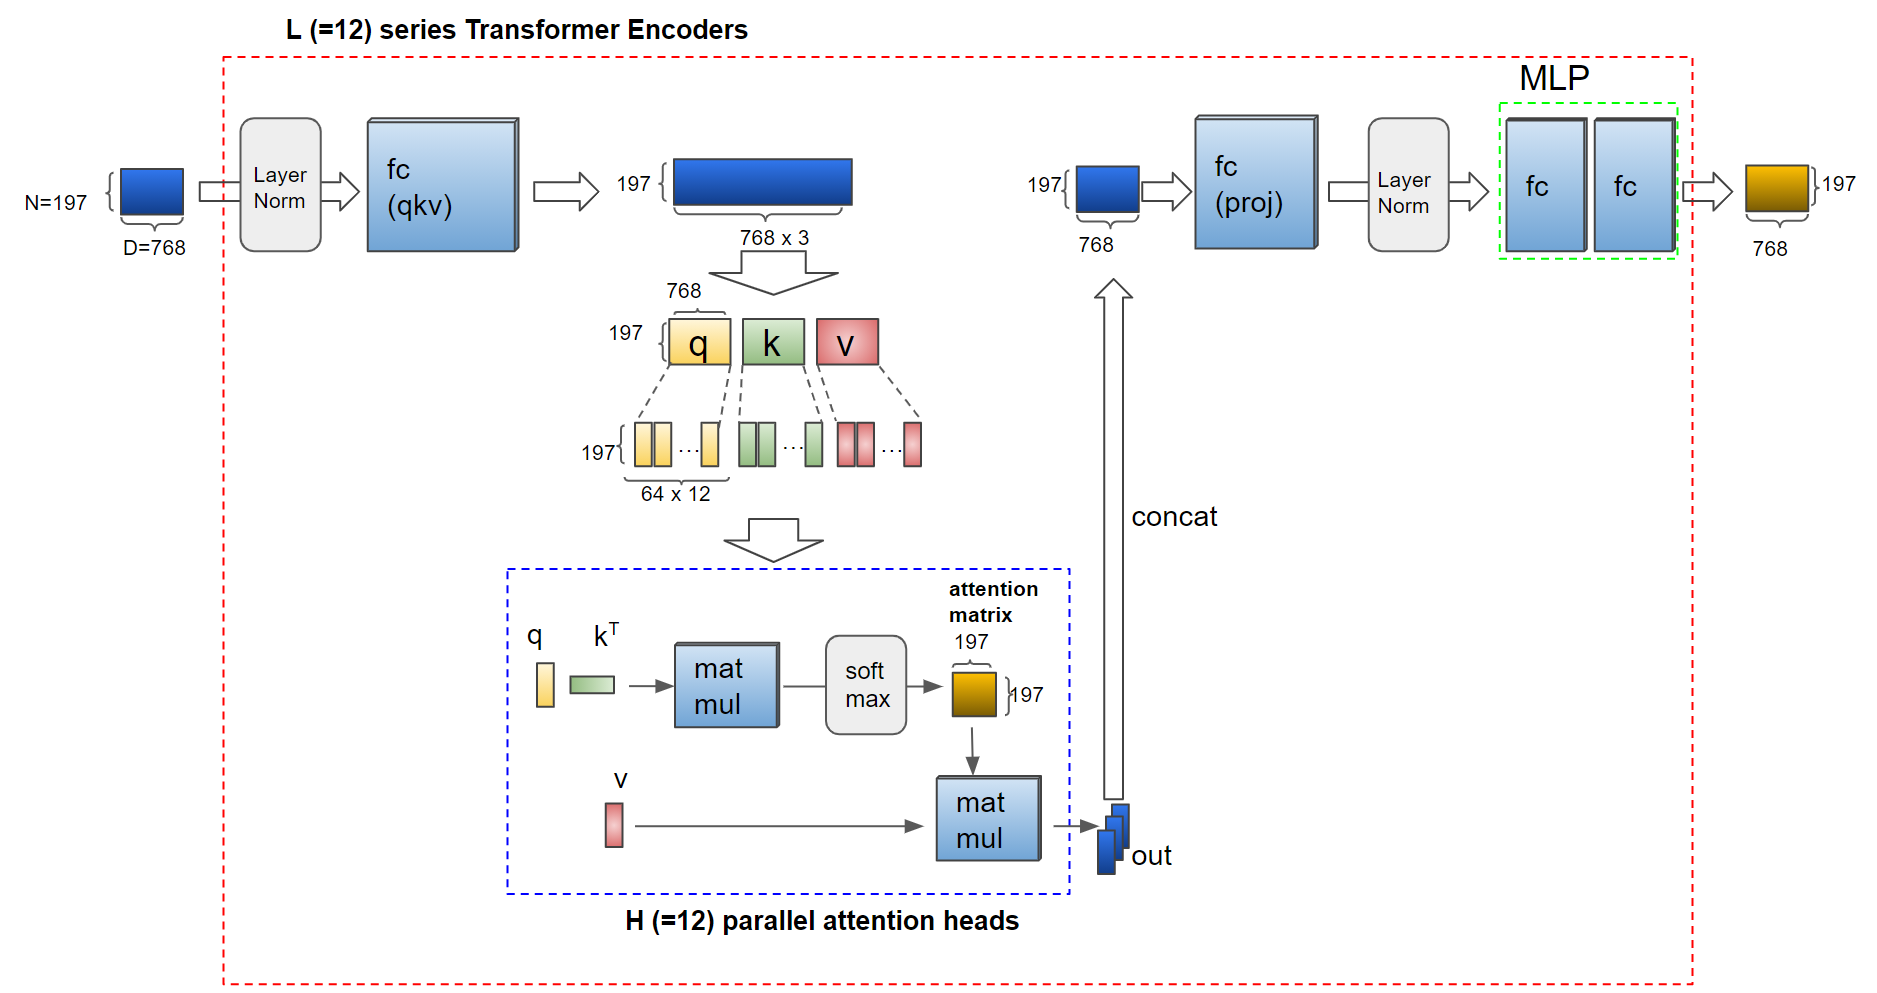
\includegraphics[width=0.8\textwidth]{figures/artificial/vit_encoder.png}
        \end{figure} 
\end{frame}
\begin{frame}{ViT: algorithm for sampling neuron output}
    \begin{figure}[H]
\centering
\begin{subfigure}[b]{0.45\textwidth}
    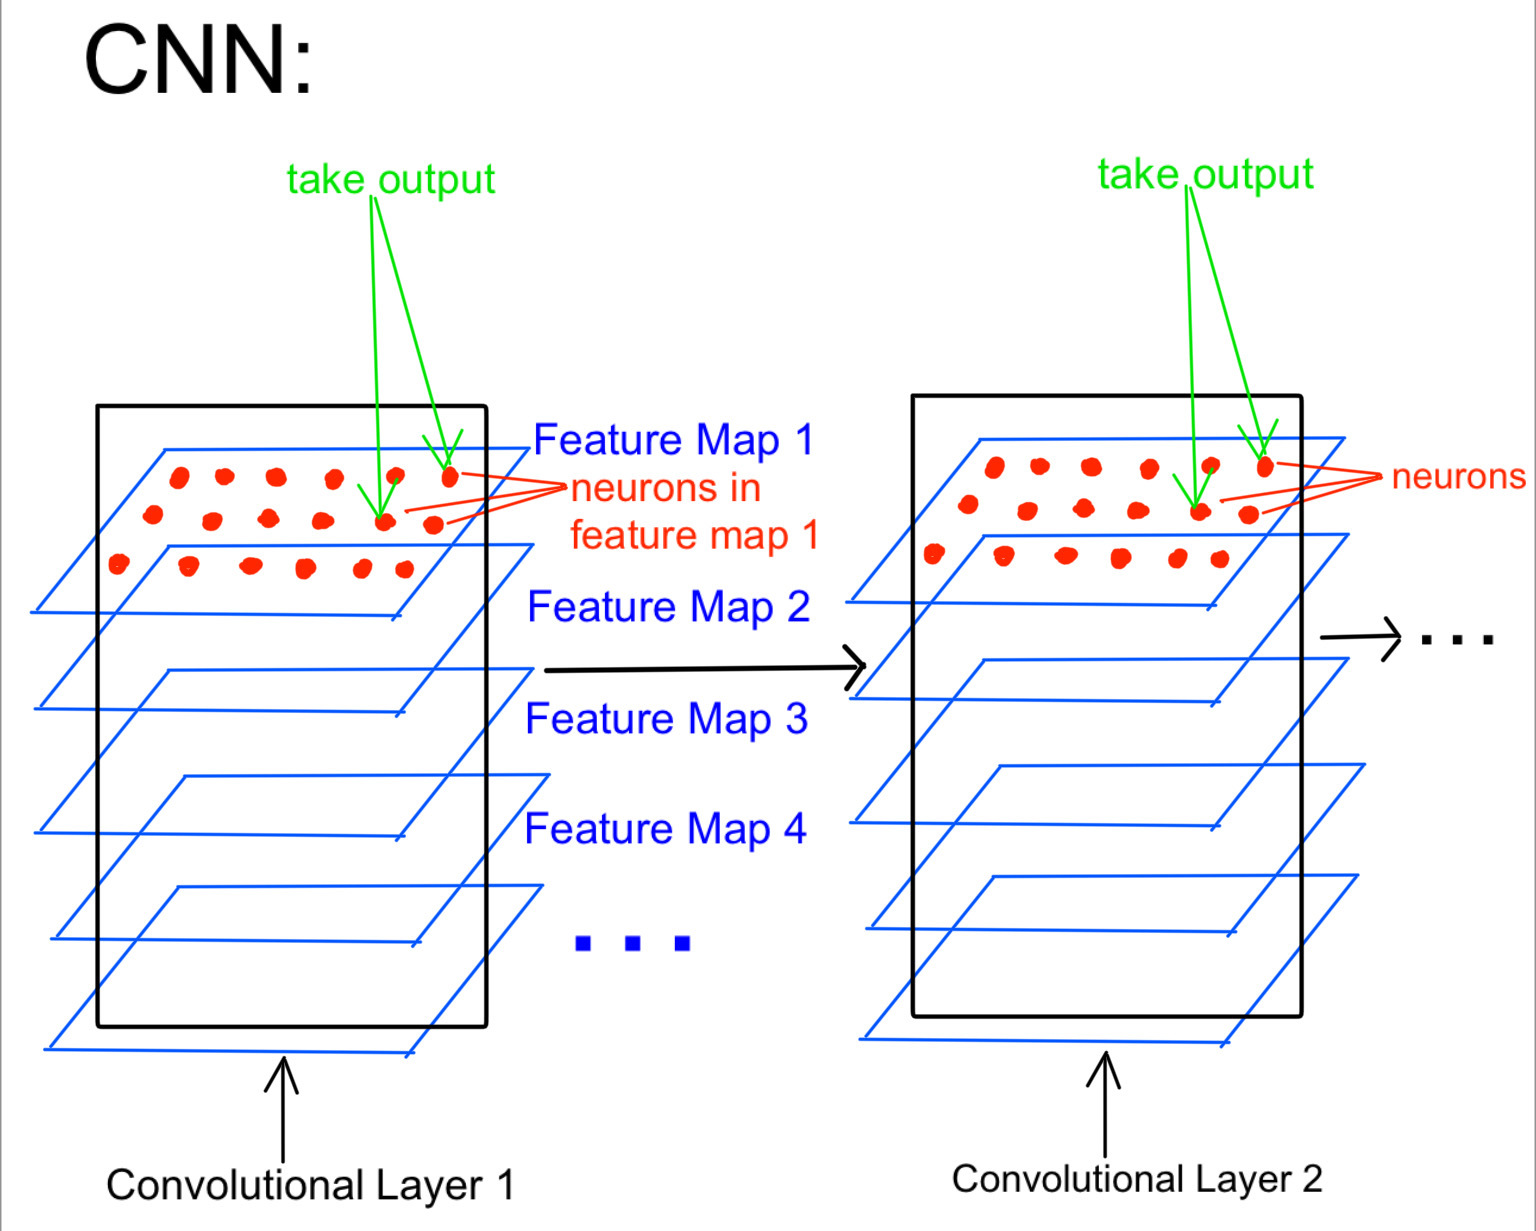
\includegraphics[width=\textwidth]{figures/artificial/cnn-tensor.jpg}
    \caption{Taking neuron output from CNN to build the corresponding neural tensor.}
\end{subfigure}
\hfill
\begin{subfigure}[b]{0.5\textwidth}
    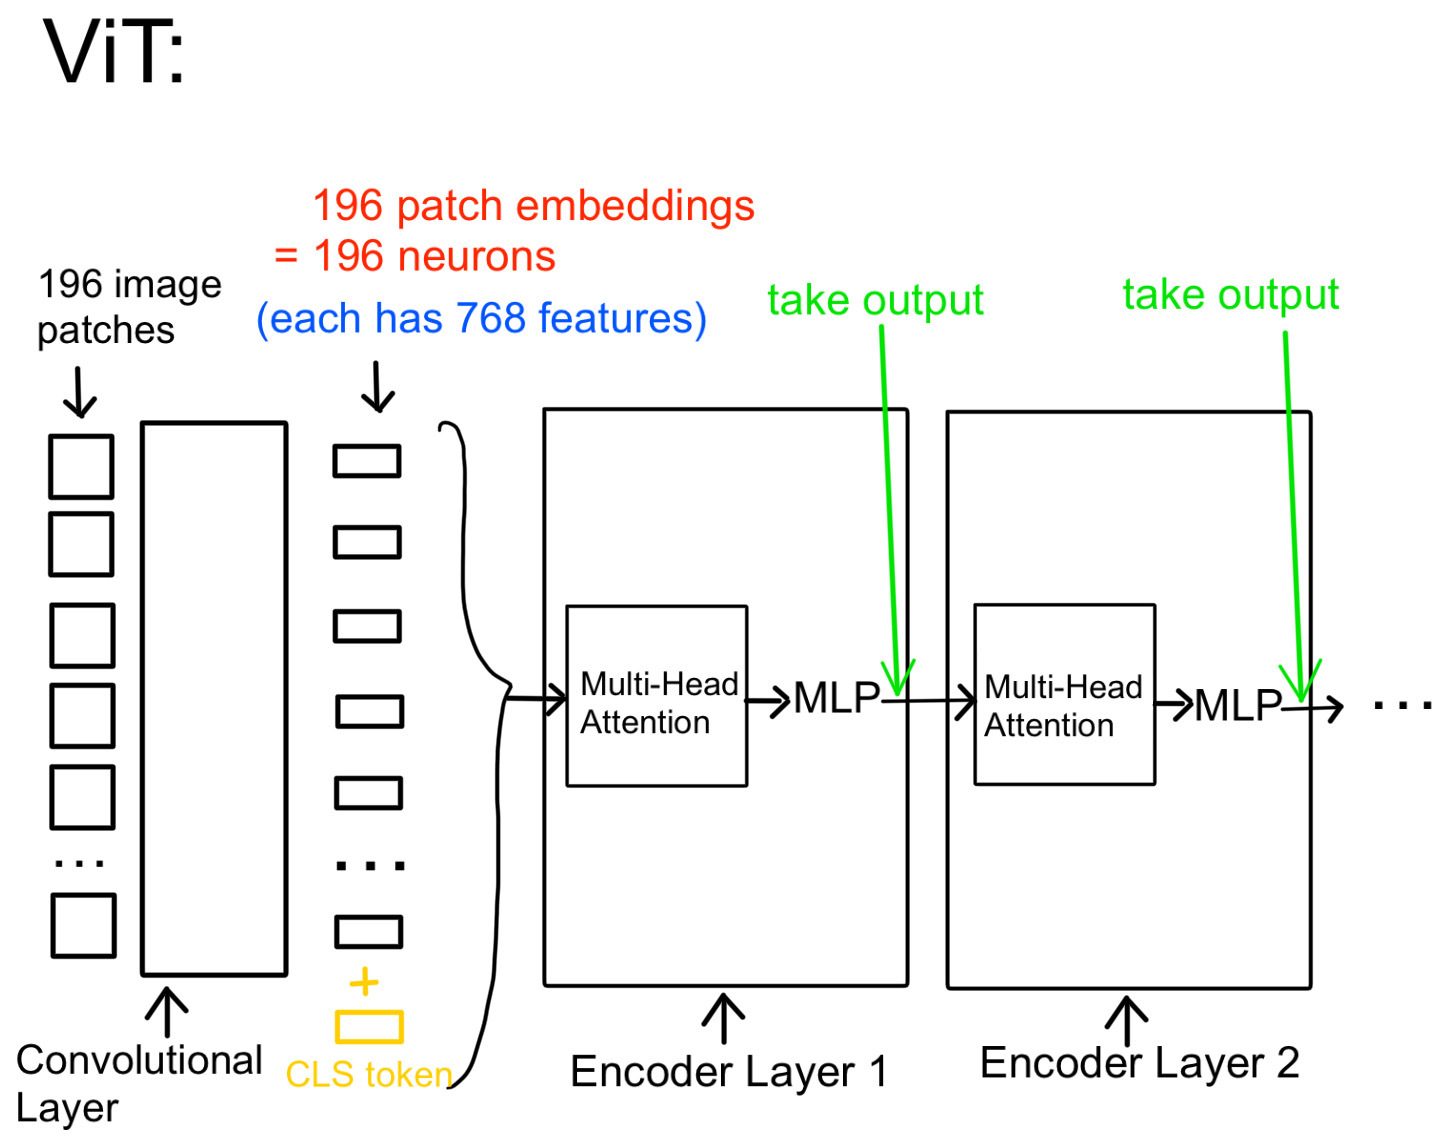
\includegraphics[width=\textwidth]{figures/artificial/vit-tensor.jpg}
    \caption{Taking neuron output from ViT to build the corresponding neural tensor.}
\end{subfigure}
\end{figure} 
\end{frame}
\begin{frame}{ViT: neural manifold}
\begin{itemize}
    \item Similar to CNN, the neural manifold is discontinuous, suggesting a neural circuit with limited inter-connectivity.
    % \item ViT neural circuit form isolated subcircuits with low inter-connectivity.
    \item Unlike CNN, the clusters remain the same shape through the layers
    \item This aligns with the findings in \cite{coatnet_2021}, \cite{raghu_vision_2021}: convolution receptive fields are highly local and grow gradually; self-attention has global receptive field and more uniform representations between shallow and deep layers.
\end{itemize}

    \begin{minipage}[t]{.45\linewidth}  
    \begin{figure}
            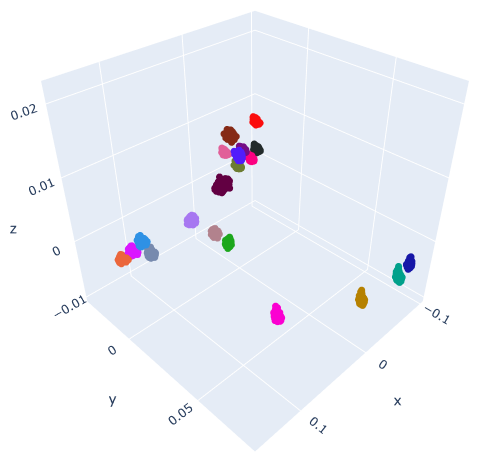
\includegraphics[width=0.7\textwidth]{figures/embeddings/vit-2d-layer1.png}
             \caption{ViT encoder layer 1 neural manifold.}
        \end{figure} 
    \end{minipage}
      \begin{minipage}[t]{.45\linewidth}   
      \begin{figure}         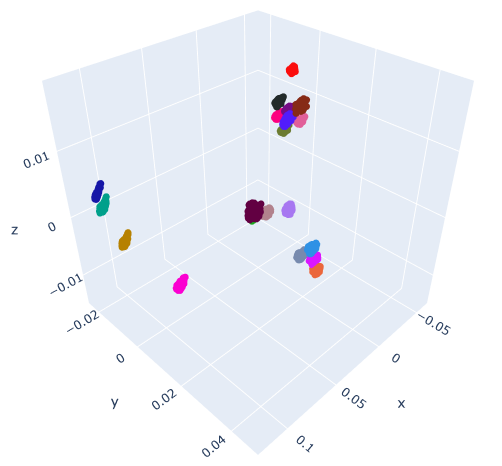
\includegraphics[width=0.6\textwidth]{figures/embeddings/vit-2d-layer12.png}
       \caption{ViT encoder layer 12 neural manifold.}
            \end{figure} 
    \end{minipage}
\end{frame}
\begin{frame}{Qualitative comparison: neural manifold}
        \begin{minipage}[b]{.45\linewidth}  
    \begin{figure}
            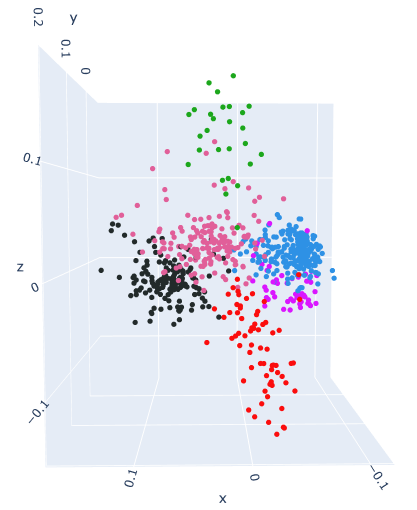
\includegraphics[width=0.6\textwidth]{figures/biological/retina-manifold.png}
            \caption{Retina.}
        \end{figure} 
    \end{minipage}
      \begin{minipage}[b]{.45\linewidth}   
      \begin{figure}         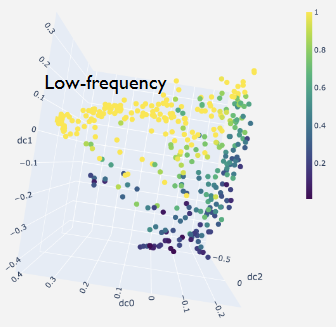
\includegraphics[width=0.6\textwidth]{figures/biological/v1-manifold-luciano.PNG}
      \caption{V1 \cite{dyballa_manifold_2021}.}
            \end{figure} 
    \end{minipage}
    
        \begin{minipage}[t]{.45\linewidth}  
    \begin{figure}
            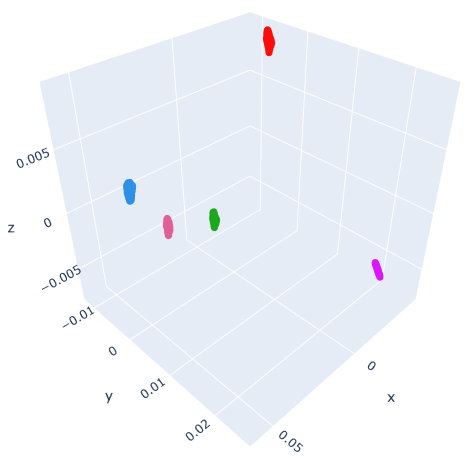
\includegraphics[width=0.7\textwidth]{figures/embeddings/VGG16-2D-block1.png}
            \caption{CNN.}
        \end{figure} 
    \end{minipage}
      \begin{minipage}[t]{.45\linewidth}   
      \begin{figure}         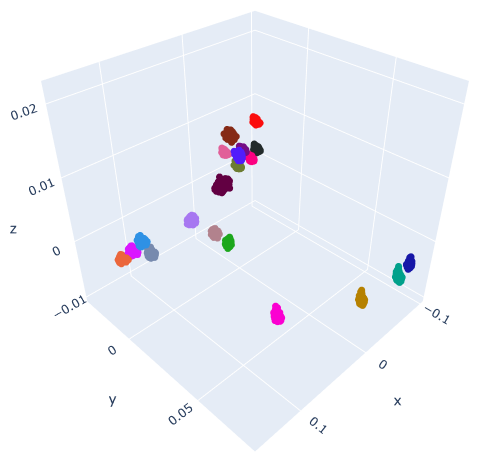
\includegraphics[width=0.7\textwidth]{figures/embeddings/vit-2d-layer1.png}
      \caption{ViT.}
            \end{figure} 
    \end{minipage}
\end{frame}
\begin{frame}{Quantitative comparison: mean flow ratio ($\phi_G$)}
\begin{figure}[H]
\centering
\begin{subfigure}[b]{0.3\textwidth}
        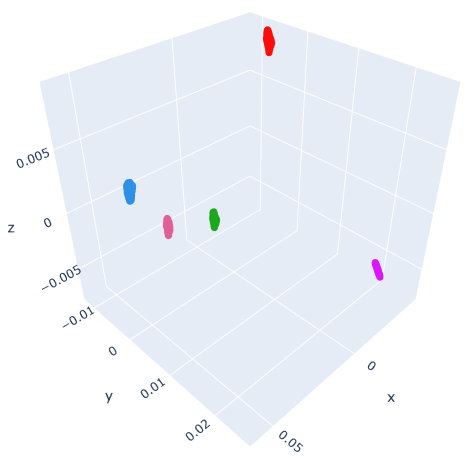
\includegraphics[width=\textwidth]{figures/embeddings/VGG16-2D-block1.png}
        \caption{$\phi_G = 0.27$ for CNN.}
\end{subfigure}
\hfill
\begin{subfigure}[b]{0.3\textwidth}
        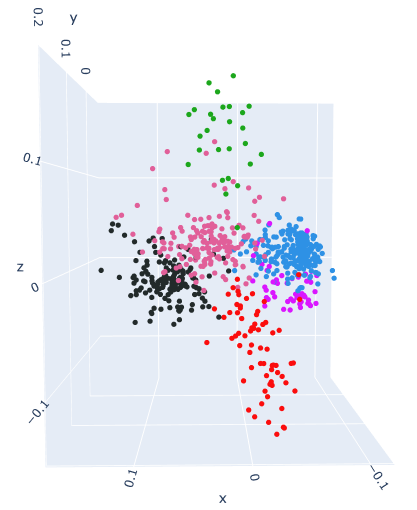
\includegraphics[width=\textwidth]{figures/biological/retina-manifold.png}
        \caption{$\phi_G = 0.56$ for retina.}
\end{subfigure}
\hfill
\begin{subfigure}[b]{0.3\textwidth}
        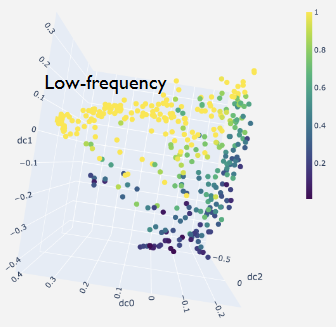
\includegraphics[width=\textwidth]{figures/biological/v1-manifold-luciano.PNG}
        \caption{$\phi_G = 0.91$ for V1 \cite{dyballa_manifold_2021}.}
\end{subfigure}
\end{figure} 
The quantitative comparison aligns with our qualitative comparison!
\end{frame}
\begin{frame}{Hypothesis: adding recurrence}
\begin{itemize}
    \item Both CNN and ViT yield discontinuous neural manifold like the retina (limited connectivity in their underlying neural circuits).
    \item Hypothesis: their feed-forward property leads to this limited connectivity. Incorporating recurrent connections might increase the continuity of the neural manifold (and hence connectivity of the neural circuit).
    \item Next model to investigate: CRNN.
\end{itemize}    
\begin{figure}[H]
\centering
    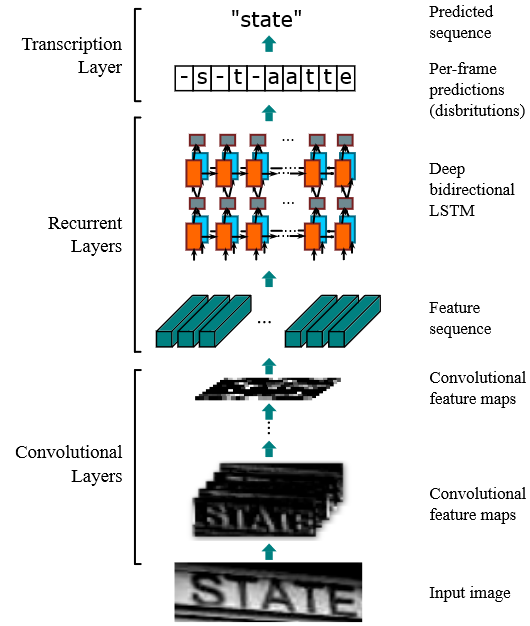
\includegraphics[width=0.35\textwidth]{figures/artificial/crnn.PNG}
\caption{Structure of CRNN.}
\end{figure}
\end{frame}

\begin{frame}{CRNN neural manifold}
\begin{itemize}
    \item After adding recurrent layers to the base CNN model, clusters of neurons share significant overlaps. 
    \item CRNN neural manifold is more continuous than CNN, suggesting greater inter-connectivity in the neural circuit. 
\end{itemize}
    \begin{figure}[H]
\centering
    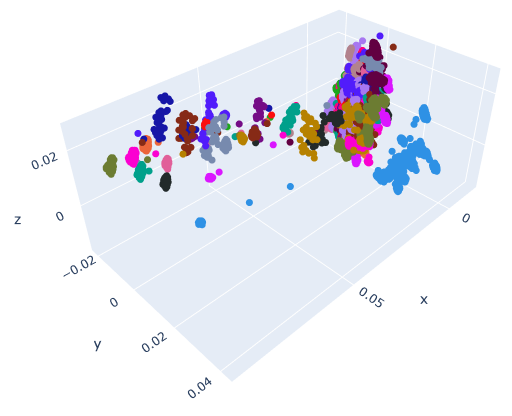
\includegraphics[width=0.5\textwidth]{figures/embeddings/crnn-2d-layer1.png}
\caption{Neural manifold for CRNN (shallow layer).}
\end{figure}
\end{frame}



\section[Conclusions]{Conclusions and Future Directions}
\begin{frame}{Conclusions}
\begin{itemize}
    \item \textcolor{blue}{\textit{How do computer vision models (VGG16, ViT, and CRNN) compare to biological vision, at retina and V1, in terms of their respective neural circuits?}}
    
    \textbf{Conjecture 1.} The underlying neural circuits in feed-forward networks, including CNN and ViT, are closer to that in retina than that in V1. Thus, contrary to popular belief, current computer vision models are poor approximations of the neural circuit of visual cortex.
    
    \item \textcolor{blue}{\textit{What specific mechanisms are important in causing such differences and/or similarities?}}
    
    \textbf{Conjecture 2.} Incorporating recurrent mechanisms in computer vision models seems to be crucial in increasing the connectivity of the underlying neural circuits. 
\end{itemize}
\end{frame}
\begin{frame}{Highlights}
During the project, we have made the following original contributions:
\begin{enumerate}
    \item conducted new computational experiments on neural data in the retina,
    \item developed original algorithms to investigate the manifold structure of CNN, ViT, CRNN,
    \item compared and analyzed (both qualitatively and quantitatively) the manifold structure of CNN, ViT, and CRNN, against that of the neurobiological networks in retina and V1,
    \item new results that have significant implications for the fields of neuroscience and computer vision.
\end{enumerate}
\end{frame}

\begin{frame}{Limitations and Future Directions}
\begin{itemize}
    
    \item Building on the empirical results, we can further develop a theoretical analysis on how recurrent connections increase the connectivity of neural circuits. 
    \item Simply adding recurrent layers has limited effect. We are currently testing other CV models where recurrent connections plays a more prominent role, in particular $\gamma$-net \cite{serre-recurrence} that adds recurrence directly onto the convolutional layers.
    \item It would be of interest to extend the mean flow ratio analysis to different recurrent models for a more precise comparison. 
\end{itemize}
\end{frame}

\begin{frame}{Acknowledgements}
I would like to thank my supervisor Prof.~Francesca Spagnuolo  and co-supervisor and mentor Prof.~Steven W. Zucker and Dr.~Luciano Dyballa for their generous guidance and advice. They have made possible the many serendipitous moments in this project. 
\end{frame}
\section{References}
\begin{frame}[allowframebreaks]{References}
\tiny
\bibliographystyle{plain}
\bibliography{biblio}
\end{frame}
\section[Q \& A]{Thank you for listening! Any questions?}
\begin{frame}{Which one is the neural manifold?}
    Finding the true CP rank of a $n$-tensor is NP-hard for $n \in \mathbb{Q}$. Thus, we do not know the true CP rank of the neural manifold. The only thing we can do is to approximate the rank using repeated dimensionality reduction steps. The neural manifold is a lower-dimensional manifold spanned by the independent neural patterns, which is thus the best intermediate representation of the original neuron output in the sense that it requires the least number of dimensions while still preserving the structure of the original neuron output. Both the neural tensors and the 3D projection plots are only approximations of the true neural manifold (since we DO NOT know the true intrinsic dimension!)
\end{frame}
\begin{frame}{More on neural manifold}
    Neural manifold is an intermediate step from the neural output towards inferring the neural circuits. On the neural manifold, each point represents a neuron. The distance between a pair of points indicates how similar the firing patterns of the corresponding neurons are, and equivalently, how likely they participate in the same neural circuit. To infer the (unknown) neural circuit from a neural manifold (known), we note that there are three possible cases: if neurons were sampled 
\begin{enumerate}
    \item from a collection of isolated neural circuits (decomposable networks), then the neurons would have distinct stimuli preferences, yielding a discontinuous neural manifold.
    \item from overlapping neural circuits (partially decomposable networks), most neurons would respond to multiple stimuli, leading to a smooth transition in stimuli preferences and a continuous neural manifold. 
    \item from fully connected neural circuits (non-decomposable networks),  all neurons would respond to all stimuli, and there would be no stimuli preferences across groups of neurons. This would yield a zero-dimensional (i.e., degenerate) manifold.
\end{enumerate}
\end{frame}
\begin{frame}{Recurrence}
    However, recent research starts to suggest that these feed-forward neural networks fail to model various key features in early primate vision  \cite{oreilly_recurrent_2013}, \cite{spoerer_recurrent_2017}, \cite{ricci_same-different_2018}, \cite{kietzmann_recurrence_2019}, \cite{van_bergen_going_2020}.
    
    In addition, more recently, recurrent models of the visual system has inspired a new topic of research that focus on applying the idea behind recurrence model to show and/or address limitations of computer vision models. Among other similar works (\cite{oreilly_recurrent_2013}, \cite{spoerer_recurrent_2017},  \cite{kietzmann_recurrence_2019}, \cite{van_bergen_going_2020}), two notable recent works are \cite{ricci_same-different_2018}, which proposed that feedback mechanisms including attention and perceptual grouping are key to visual relational reasoning tasks and \cite{kietzmann_recurrence_2019}, which showed that recurrence is necessary to model the representational dynamics in the visual system.

\end{frame}

\begin{frame}{Visual reasoning}
    A growing number of research starts to reveal tasks that biological vision excels at while the state-of-the-art computer vision models fail. One notable example is that CNN is highly inferior to human vision in solving visual problems that involve relational reasoning \cite{glorot-bengio-difficulty}, such as recognizing same-different relations in images \cite{ricci_same-different_2018}, categorizing images based on the constituent parts \cite{visual-categorization}, and comparing features in images  \cite{cnn-human-abstraction}. The hope is that with a rigorous comparison, we can discover the specific mechanisms responsible for certain desired features of biological vision that the current computer vision models are lacking and adapt those mechanisms into computer vision models with relevant computational constraints in mind.
\end{frame}

\begin{frame}{Algorithm for NTF for retina tensor}
\begin{algorithm}[H]
\caption{Algorithm for NTF on retina tensor.}\label{alg:factors-retina}
\KwData{Neural tensor for retina.}
\KwResult{$R$ tensor factors for retina.}
\DontPrintSemicolon
import data as X, X = tensor(X) \;
chosen rank, R = 35 \;
n\_repetitions = 10, initialize errors with zeros \; 
\For{r from 1 to R}{
\For{rep from 1 to n\_repetitions}{
NTF: M = cp\_opt(X, r, 'init', 'rand' , 'lower', 0) \;
error = norm(X - tensor(M)) / norm(X); \;
add error to the array of errors \;
}
}
F\_neuron = M.u\{1\}, F\_stimuli = M.u\{2\}, F\_time = M.u\{3\} \;
save the factors \;
\end{algorithm}
\end{frame}

\begin{frame}{Algorithm for computing the mean flow ratio}
\begin{algorithm}[H]
\caption{Algorithm for computing the mean flow ratio.}\label{alg:mean-flow-ratio}
\DontPrintSemicolon
\KwData{points on the neural manifold, $\xx_1, \dots, \xx_N \in \mathcal{M}$.}
\KwResult{mean flow ratio for the neural manifold, $\phi_G$.}
kernel bandwidth, $\epsilon \coloneqq \frac{1}{N}\sum_{i=1}^N \min_{j: \xx_j \neq \xx_i}\|\xx_i - \xx_j\|^2$\;
Gaussian kernel\footnote{In fact, we can choose any symmetric, positive semi-definite similarity kernel. But Gaussian kernel gives a physically intuitive construction as it effectively considers a ball of radius $\epsilon$ around each data point.}, $k(\xx_i, \xx_j) = \exp(-\|\xx_i - \xx_j\|^2/\epsilon)$ \;
weight matrix $W, W_{i, j}\coloneqq {k_\epsilon}(\xx_i, \xx_j)$\;
degree of node $\xx_i$, $d(\xx_i) \coloneqq \sum_{j=1}^N W_{i,j}$\;
anisotropic Gaussian kernel, $\Tilde{k_\epsilon}(\xx_i, \xx_j) \coloneqq \frac{k_\epsilon(\xx_i, \xx_j)}{d(\xx_i)d(\xx_j)}$ \;
anisotropic weight matrix,$\Tilde{W}, \Tilde{W}_{i, j}\coloneqq \Tilde{k_\epsilon}(\xx_i, \xx_j)$\;
build graph $G = (V, E)$, weight of the edge ($\xx_i$, $\xx_j$) is $\Tilde{W}_{i, j}$ \;
\end{algorithm}
\end{frame}

\begin{frame}{(Cont.)}
\begin{algorithm}[H]
\caption{Algorithm for computing the mean flow ratio (cont.).}\label{alg:mean-flow-ratio-cont}
\DontPrintSemicolon
edge resistance, $R_{i, j} = 1/\Tilde{W}_{i, j}$ \;
compute effective resistance $R^{\text{eff}}_{i, j}$, using \cite{effective-resistance}\;
effective conductance, $C^{\text{eff}}_{i, j} = 1/R^{\text{eff}}_{i, j}$\;
build graph $G_C$, weight of the edge ($\xx_i$, $\xx_j$) is $C^{\text{eff}}_{i, j}$  \;
\For{i from 1 to N}{
\For{j from 1 to N, $j\neq i$}{
SumAll += \text{maxflow}(i, j)\;
}
\For{k: k is a neighbor of i}{
SumNeighbors += \text{maxflow}(i, k)
}
flow ratio of node $\xx_i$, $\rho_i$ = SumAll/SumNeighbors\;
}
mean flow ratio of graph $G$, $\phi_G = \sum_{i=1}^N \rho_i.$
\end{algorithm}
\end{frame}


\begin{frame}{Algorithm for sampling neurons from CNN}
\begin{algorithm}[H]
\caption{Algorithm for CNN artificial neural tensor.}\label{alg:cnn-tensor}
\DontPrintSemicolon
% Set Function Names
%   \SetKwFunction{FShifts}{apply\_all\_shifts}
  \SetKwFunction{FOutput}{compute\_neuron\_output}
  \SetKwFunction{FStimuli}{show\_stimuli}
% Write Function with word ``Function''
%   \SetKwProg{Fn}{Function}{:}{}
%   \Fn{\FShifts{$image$, $shift\_step$}}{
%         add the original image to image\_all\_shifts\;
%         \For{i from 0 to \# vertical shifts}{
%         shift the image vertically by shift\_step\;
%         add the shifted image to image\_all\_shifts\;
%             \For{j from 0 to \# horizontal shifts}{
%             shift the image horizontally by shift\_step\;
%             add the shifted image to image\_all\_shifts\;
%             }
%         }
%   }
  \SetKwProg{Fn}{Function}{:}{}
  \Fn{\FOutput{$model$, $image\_all\_shifts$}}{
        \For{layer in all convolutional layers}{
        pass the image through the model\;
        take the neuron output from the specified layer after ReLU\;
        % , of shape (\# shifts, \# rows, \# columns, \# feature\_maps)\;
        % \# neurons in each feature map = \# rows * \# columns\;
        (optional) remove the neurons at the edges\;
        compute the average neuron output in each feature map\;
        select the feature maps with highest average \;
        normalize the neuron outputs in each feature map\;
        }
  }
  \end{algorithm}
\end{frame}
  

\begin{frame}{Algorithm for sampling neurons from ViT}
    \begin{algorithm}[H]
\caption{Algorithm for ViT artificial neural tensor.}\label{alg:vit-tensor}
\DontPrintSemicolon
% Set Function Names
  \SetKwFunction{FOutput}{compute\_neuron\_output}
  \SetKwProg{Fn}{Function}{:}{}
  \Fn{\FOutput{$model$, $image\_all\_shifts$}}{
        \For{layer in all encoder layers}{
        pass the image through the model\;
        take the neuron output from the specified layer\;
        apply ReLU activation on the neuron output\;
        compute the average of neuron outputs in each feature\;
        select the feature maps with highest average \;
        normalize the neuron outputs in each feature map\;
        }
  }
\end{algorithm}
\end{frame}
\begin{frame}{CNN: spatial ordering of neurons is preserved}
The spatial ordering of neurons' receptive fields are continuously mapped onto the manifold. 
\begin{figure}
            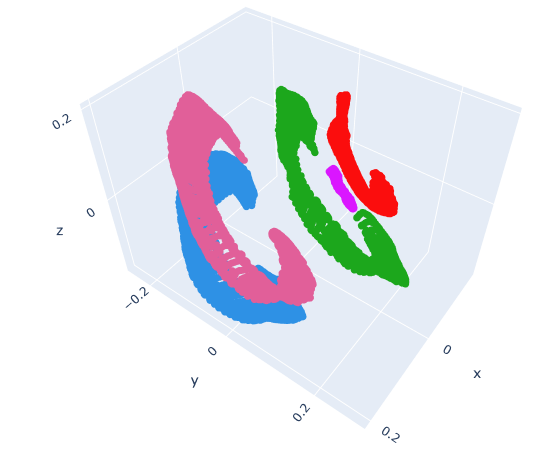
\includegraphics[width=0.4\textwidth]{figures/embeddings/VGG16-3D-block1.png}
            \caption{VGG16 block 1 neural manifold with spatial order preserved.}
        \end{figure} 
    \begin{minipage}[t]{.45\linewidth}  
    \begin{figure}
            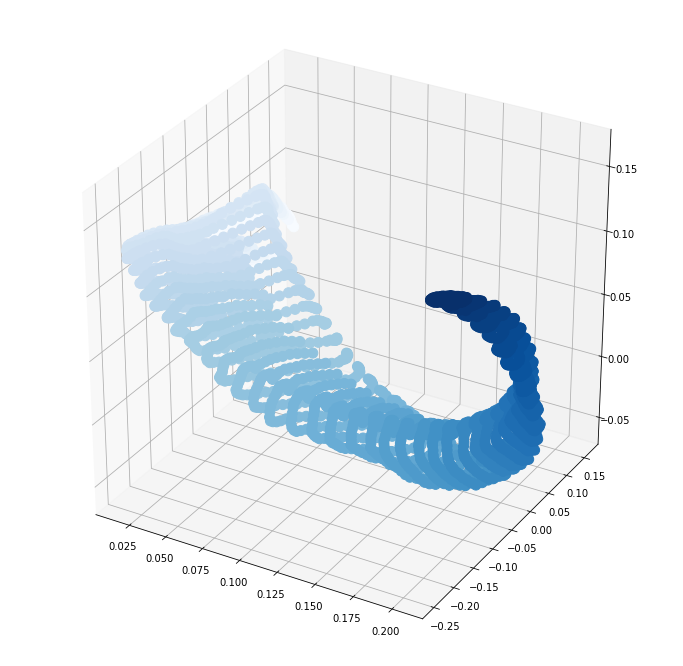
\includegraphics[width=0.5\textwidth]{figures/embeddings/vgg16-spatial1.png}
            \caption{First cluster of neurons organized by vertical order.}
        \end{figure} 
    \end{minipage}
      \begin{minipage}[t]{.45\linewidth}   
      \begin{figure}         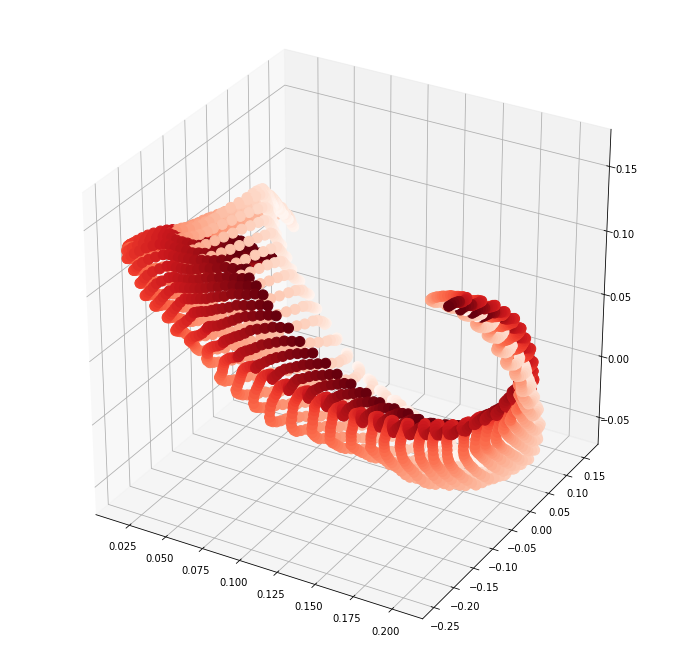
\includegraphics[width=0.5\textwidth]{figures/embeddings/vgg16-spatial2.png}
      \caption{First cluster of neurons organized by horizontal order.}
            \end{figure} 
    \end{minipage}
\end{frame}
\begin{frame}{ViT: spatial ordering of neurons is preserved}
\begin{figure}
            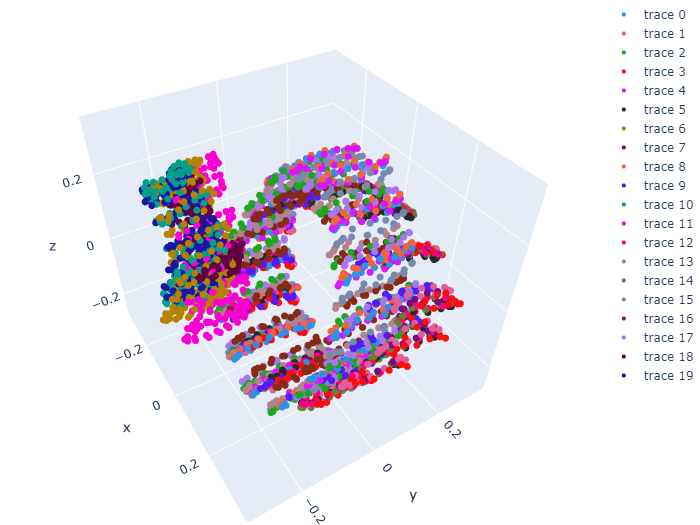
\includegraphics[width=0.4\textwidth]{figures/embeddings/vit-3d-layer1.png}
            \caption{ViT encoder layer 1 neural manifold with spatial order preserved.}
        \end{figure} 
    \begin{minipage}[t]{.45\linewidth}  
    \begin{figure}
            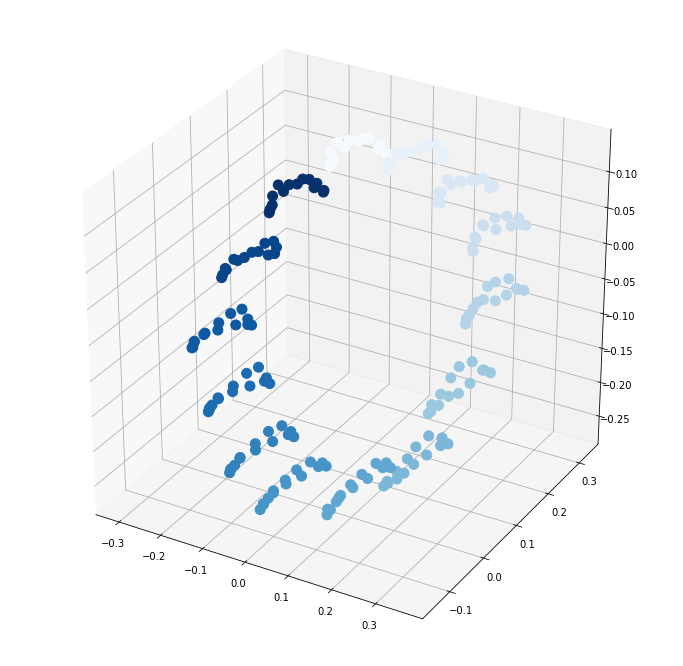
\includegraphics[width=0.5\textwidth]{figures/embeddings/vit-spatial1.png}
            \caption{First cluster of neurons organized by vertical order.}
        \end{figure} 
    \end{minipage}
      \begin{minipage}[t]{.45\linewidth}   
      \begin{figure}         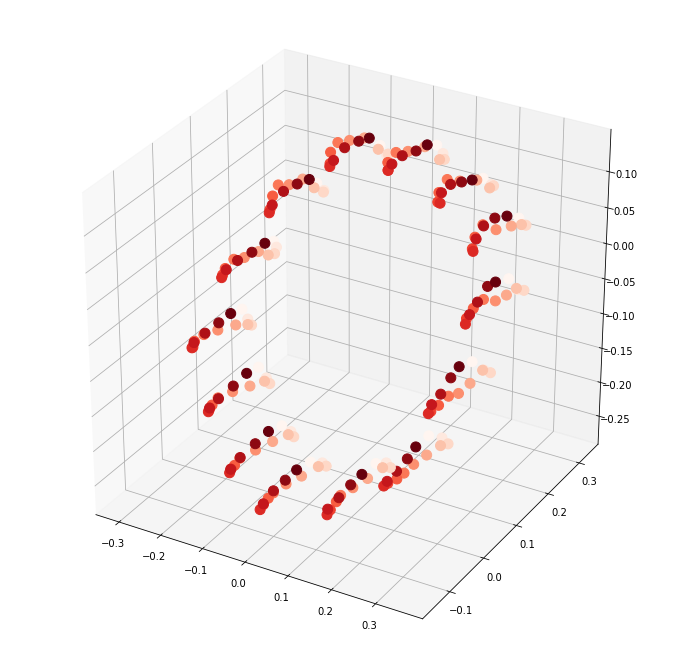
\includegraphics[width=0.5\textwidth]{figures/embeddings/vit-spatial2.png}
      \caption{First cluster of neurons organized by horizontal order.}
            \end{figure} 
    \end{minipage}
\end{frame}

\begin{frame}[allowframebreaks]{Remarks}
\begin{rmk}
For ease of reference, we also use the term ``neural manifold" for the point-cloud of data points with an underlying manifold structure. In addition, neural manifolds from real neural data are often no longer ``manifolds” in a mathematical sense, due to the sparse input sampling and the presence of neural noise. 
\end{rmk}
    
\begin{rmk}
At first it might seem that using different stimuli for biological and artificial neural networks will lead to an unfair comparison. However, this approach is appropriate for the following reason: The mouse visual system was trained on the flow stimuli is shown to resemble the naturalistic visual information that the mouse's vision has adapted to\footnote{Based on the paper that proposed flow stimuli \cite{visual-flow}, flow stimuli are more like what the mouse would encounter in the natural world than are sine-wave gratings but is more tractable for analysis than are natural images.}. The visual stimuli for VGG16 model came from the same data set that it is trained on (ImageNet). Thus, in both cases, the visual stimuli are similar to what the respective network was trained to recognize.
\end{rmk}

\begin{rmk}
On line 5, we need to impose ReLU\footnote{ReLU: Rectified Linear Unit \cite{relu}.} activation to make the neuron output non-negative. The non-negative constraint is desired because the tensor factors from NTF are more interpretable. The pre-trained ViT uses GELU\footnote{GELU: Gaussian Error Linear Unit \cite{gelu}.} as the activation function. This results in negative values and would prevent us from using non-negative tensor decomposition. Fortunately, the negative portion of GELU is negligible given the purpose of our investigation, which justifies this step.
\end{rmk}

\end{frame}


\begin{frame}[allowframebreaks]{Analogy}

\textbf{``Visual stimuli" in CNN}

Analogous to the flow stimuli in lab experiments, the ``visual stimuli" for CNN are natural images of different objects selected from the benchmark dataset ImageNet \cite{deng2009imagenet}. To keep the size of the artificial neural tensor manageable, we randomly selected 20 images from four classes as the visual stimuli. In order to simulate the movement of flow stimuli over time, we create multiple shifts of the original image in vertical and horizontal direction, with the shift step equal to the size of the filter. 
    % add image
    \begin{figure}[H]
        \centering
            \includegraphics[width=0.7\textwidth]{figures/artificial/artificial-input-output.jpg}
            \caption{Computing output of one neuron unit in the CNNs given 10 input cat images.}
    \end{figure}
    
 \textbf{``Individual neuron" in CNN}
 In the lab experiments for biological neural networks, moving visual stimuli trigger spikes in the activation potential in the neurons in the retina. The individual neuron response is the firing rate of the neuron which is dependent on the  electrostatics processes that take place in the synapse. The biological neuron is coarsely modeled by the neuron unit in the CNNs. At the ``dendrite," the input is taken from the ``axons" of the connected neurons.\footnote{Note, however, that in our experiments, instead of taking the input from previously connected neuron unit, each neuron takes the image as the input.} The weight of each neuron models the synaptic process in biological neuron. At the ``cell body," all the inputs are multiplied with the weights and summed. We then add the bias term to the sum and apply the nonlinear activation to obtain the final output from the individual neuron unit at the ``axon." The parallel between biological and artificial neuron is shown in the figures below. 
\begin{figure}[H]
\centering
\begin{subfigure}[b]{0.5\textwidth}
        \includegraphics[width=0.9\textwidth]{figures/artificial/neuron.png}
        \caption{An individual neuron in biological neural networks. Adapted from \cite{cs231n}.}
\end{subfigure}
\hfill
\begin{subfigure}[b]{0.45\textwidth}
        \includegraphics[width=0.9\textwidth]{figures/artificial/neuron_model.jpeg}
        \caption{An ``individual neuron" in CNNs. Adapted from \cite{cs231n}.}
\end{subfigure}
\end{figure}
\textbf{``Receptive field" of an artificial neuron}
Each layer in the CNN has several different feature maps. Each feature map corresponds to a filter of a specific size and specific weights. The filter is essentially a matrix that, when taking inner product with the input image, give an output that highlights some specific features in the input image. To illustrate this, we can visualize the 64 feature map in the first convolutional layer of the VGG16 model, given the input image.
\begin{figure}[H]
\centering
\begin{subfigure}[b]{0.3\textwidth}
        \centering
  \includegraphics[width=0.6\textwidth]{figures/artificial/bird.jpg}
\caption{Input image. Adapted from \cite{feature_map}.}
\end{subfigure}
\hfill
\begin{subfigure}[b]{0.65\textwidth}
\centering
    \includegraphics[width=0.45\textwidth]{figures/artificial/feature_map_vgg16.png}
    \caption{Visualizing the 64 feature maps in the first convolutional layer of the VGG16 model. Adapted from \cite{feature_map}.}
\end{subfigure}
\end{figure} 

The neurons within each feature map share the same weights and each attends to a specific subregion of the image which is referred to as their receptive field. This term originated from biological vision defined as a restricted region of visual space where a stimulus could illicit responses in a retinal ganglion cell. The size of the receptive field of a neuron is the same as the filter size corresponding to the feature map in which the neuron is located. 

\textbf{``Neuron population response" in CNN}
Analogous to biological neural networks, we computed the neural output given the input image. Unlike biological neurons, most of the artificial neurons will have output of small values because most pre-trained weights decay to zero. In other words, the ``firing" of neurons in CNN will be sparse. We select the feature maps that contain the neurons with highest average firing rate.
\end{frame}


\end{document}